\newpage
\section{Class \Iclass{triangle}} % (fold)
\label{sec:class_triangle}

\subsection{Attributes of a triangle} % (fold)
\label{sub:attributes_of_a_triangle}
The triangle object is created using the \Imeth{triangle}{new} method, for example with
\begin{mybox}
   Creation  | T.ABC = triangle : new ( z.A , z.B , z.C ) |
\end{mybox}
(Refer to examples:  \ref{sub:alternate}; \ref{sub:apollonius_circle}; \ref{sub:excircles} ). Multiple attributes are then created.

\bgroup
\catcode`_=12
\small
\captionof{table}{Triangle attributes.}\label{triangle:att}
\begin{tabular}{ll}
\toprule
\textbf{Attributes}     & \textbf{Application}\\
\Iattr{triangle}{pa} &T.ABC.pa \\
\Iattr{triangle}{pb} &T.ABC.pb \\
\Iattr{triangle}{pc} &T.ABC.pc \\
\Iattr{triangle}{type} & 'triangle' \\
\Iattr{triangle}{circumcenter} & T.ABC.circumcenter; [\ref{ssub:example_triangle_attributes}
]\\
\Iattr{triangle}{centroid} &T.ABC.centroid\\
\Iattr{triangle}{incenter} &T.ABC.incenter\\
\Iattr{triangle}{orthocenter}  &T.ABC.orthocenter\\
\Iattr{triangle}{eulercenter} &T.ABC.eulercenter  \\
\Iattr{triangle}{spiekercenter} &T.ABC.spiekercenter; [\ref{ssub:example_apollonius_circle}]  \\
\Iattr{triangle}{a}& It's the length of the side opposite the first vertex  \\
\Iattr{triangle}{b}& It's the length of the side opposite the second verte\\
\Iattr{triangle}{c}& It's the length of the side opposite the third vertex \\
\Iattr{triangle}{alpha}& Vertex angle of the first vertex\\
\Iattr{triangle}{beta}& Vertex angle of the second vertex\\
\Iattr{triangle}{gamma}& Vertex angle of the third vertex\\
\Iattr{triangle}{ab}& Line defined by the first two points of the triangle\\
\Iattr{triangle}{bc}& Line defined by the last two points \\
\Iattr{triangle}{ca}&  Line defined by the last and the first points of the triangle\\
\bottomrule %
\end{tabular}
\egroup

\subsection{Triangle attributes: angles} % (fold)
\label{sub:triangle_attributes_angles}

\begin{minipage}{.6\textwidth}
\begin{Verbatim}
\begin{tkzelements}
  z.A       = point: new(0,0)
  z.B       = point: new(5,0)
  z.C       = point: new(2,3)
  T.ABC     = triangle: new (z.A,z.B,z.C)
\end{tkzelements}
\def\wangle#1{\tkzDN[2]{%
  \tkzUseLua{math.deg(T.ABC.#1)}}}
\begin{tikzpicture}
\tkzGetNodes
  \tkzDrawPolygons(A,B,C)
  \tkzLabelAngle(B,A,C){$\wangle{alpha}^\circ$}
  \tkzLabelAngle(C,B,A){$\wangle{beta}^\circ$}
  \tkzLabelAngle(A,C,B){$\wangle{gamma}^\circ$}
\end{tikzpicture}
\end{Verbatim}
\end{minipage}
\begin{minipage}{.4\textwidth}
\begin{tkzelements}
   z.A       = point: new(0,0)
   z.B       = point: new(5,0)
   z.C       = point: new(2,3)
   T.ABC     = triangle: new (z.A,z.B,z.C)
\end{tkzelements}
\def\wangle#1{\tkzDN[2]{\tkzUseLua{math.deg(T.ABC.#1)}}}
\begin{tikzpicture}
\tkzGetNodes
\tkzDrawPolygons(A,B,C)
\tkzLabelAngle(B,A,C){$\wangle{alpha}^\circ$}
\tkzLabelAngle(C,B,A){$\wangle{beta}^\circ$}
\tkzLabelAngle(A,C,B){$\wangle{gamma}^\circ$}
\end{tikzpicture}
\end{minipage}
% subsection triangle_attributes_angles (end)

\subsubsection{Example: triangle attributes} % (fold)
\label{ssub:example_triangle_attributes}
\begin{minipage}{.5\textwidth}
\begin{Verbatim}
\begin{tkzelements}
   z.A   = point: new (0 , 0)
   z.B   = point: new (4 , 0)
   z.C   = point: new (0 , 3)
   T.ABC = triangle : new (z.A,z.B,z.C)
   z.O   = T.ABC.circumcenter
   z.I   = T.ABC.incenter
   z.H   = T.ABC.orthocenter
   z.G   = T.ABC.centroid
   a     = T.ABC.a
   b     = T.ABC.b
   c     = T.ABC.c
   alpha = T.ABC.alpha
   beta  = T.ABC.beta
   gamma = T.ABC.gamma
\end{tkzelements}
\begin{tikzpicture}
   \tkzGetNodes
   \tkzDrawPolygon(A,B,C)
   \tkzDrawPoints(A,B,C,O,G,I,H)
   \tkzLabelPoints[below](A,B,O,G,I)
   \tkzLabelPoints[above right](H,C)
   \tkzDrawCircles(O,A)
   \tkzLabelSegment[sloped](A,B){\tkzUseLua{c}}
   \tkzLabelSegment[sloped,above](B,C){\tkzUseLua{a}}
\end{tikzpicture}
\end{Verbatim}
\end{minipage}
\begin{minipage}{.5\textwidth}
\begin{tkzelements}
   z.A   = point: new (0 , 0)
   z.B   = point: new (4 , 0)
   z.C   = point: new (1 , 3)
   T.ABC = triangle : new (z.A,z.B,z.C)
   z.O   = T.ABC.circumcenter
   z.I   = T.ABC.incenter
   z.H   = T.ABC.orthocenter
   z.G   = T.ABC.centroid
   a     = T.ABC.a
   b     = T.ABC.b
   c     = T.ABC.c
   alpha = T.ABC.alpha
   beta  = T.ABC.beta
   gamma = T.ABC.gamma
\end{tkzelements}  

\begin{center}
  \begin{tikzpicture}
     \tkzGetNodes
     \tkzDrawPolygon(A,B,C)
     \tkzDrawPoints(A,B,C,O,G,I,H)
     \tkzDrawCircles(O,A)
     \tkzLabelPoints[below](A,B,O,G,I)
     \tkzLabelPoints[above right](H)
     \tkzLabelPoints[above](C)
     \tkzLabelSegment[sloped](A,B){\tkzUseLua{c}}
     \tkzLabelSegment[sloped,above](B,C){\tkzUseLua{a}}
  \end{tikzpicture}
\end{center}


\end{minipage}

% subsubsection example_triangle_attributes (end)

% subsection attributes_of_a_triangle (end)

\subsection{Methods of the class triangle} % (fold)
\label{sub:methods_of_the_class_triangle}

\bgroup
\catcode`_=12
\small
\begin{minipage}{\textwidth}
\captionof{table}{triangle methods.}\label{triangle:met}
\begin{tabular}{lll}
\toprule
\textbf{Methods} & \textbf{Comments}  &    \\
\midrule
\Imeth{triangle}{new} (a, b ,c) & |T.ABC = triangle : new (z.A,z.B,z.C)|& [\ref{sub:triangle_attributes_angles}] \footnote{|T| or |T.name| with what you want for name, is possible.}  \\
\midrule 
 \textbf{Points} &&\\
\midrule 
\Imeth{triangle}{lemoine\_point ()} &  |T.ABC : lemoine_point ()| intersection of the symmedians & [\ref{ssub:method_imeth_line_isosceles}]\\

\Imeth{triangle}{symmedian\_point ()}  & Lemoine point  or the Grebe point& [\ref{ssub:method_imeth_triangle_symmedial}] \\

\Imeth{triangle}{lemoine\_point ()}  & symmedian point  or the Grebe point& [\ref{ssub:method_imeth_triangle_symmedial}] \\

\Imeth{triangle}{bevan\_point ()}  &  Circumcenter of the excentral triangle& [\ref{ssub:methods_imeth_triangle_bevan_circle_and_imeth_triangle_bevan_point}
]\\

\Imeth{triangle}{mittenpunkt\_point ()}  &  Symmedian point of the excentral triangle& [\ref{ssub:method_imeth_triangle_mittenpunkt}]\\

\Imeth{triangle}{gergonne\_point ()}  & Intersection of the three cevians that lead to the contact points& [\ref{ssub:gergonne_point}]\\

\Imeth{triangle}{nagel\_point () } & Intersection of the three cevians that lead to the extouch points& [\ref{ssub:method_imeth_triangle_nagel__point}]\\

\Imeth{triangle}{feuerbach\_point () } & The point at which the incircle and euler circle are tangent.& [\ref{ssub:method_imeth_triangle_feuerbach}]\\

\Imeth{triangle}{spieker\_center ()} &  Incenter of the medial triangle& [\ref{sub:apollonius_circle_v1_with_inversion}]\\

\Imeth{triangle}{barycentric (ka,kb,kc)} & |T.ABC: barycentric (2,1,1)| barycenter of |({A,2},{B,1},{C,1}) |&Remark \footnote{The function \code{barycenter} is used to obtain the barycentre for any number of points }\\

\Imeth{triangle}{base (u,v)  }  &  |z.D = T.ABC: base(1,1)| \tkzar ABDC is a parallelogram  & [\ref{ssub:method_imeth_triangle_base}] \\
\Imeth{triangle}{trilinear (u,v,w)  }  &  |z.D = T.ABC: trilinear(1,1,1)| \tkzar ABDC parallelogram  & [\ref{ssub:method_imeth_triangle_trilinear}] \\

\Imeth{triangle}{projection (p) }   &  Projection of a point on the sides &[\ref{sub:euler_relation}; \ref{ssub:method_imeth_triangle_projection}]\\

\Imeth{triangle}{euler\_points () } & Euler points of euler circle  & [\ref{ssub:method_imeth_triangle_euler__points}] \\

\Imeth{triangle}{nine\_points () }   & 9 Points of the euler circle & [\ref{ssub:method_imeth_triangle_nine__points}] \\

\Imeth{triangle}{parallelogram ()} & |z.D = T.ABC : parallelogram ()| \tkzar ABCD parallelogram& [\ref{sub:director_circle}]\\
\midrule
 \textbf{Lines} &&\\
\midrule 
\Imeth{triangle}{altitude (n) }  & |L.AHa = T.ABC : altitude () | n empty or 0  line from $A$  
\footnote{|z.Ha = L.AHa.pb| recovers the common point of the opposite side and altitude. The method |orthic| is usefull. If you don't need to use the triangle object several times, you can obtain a bisector or a altitude with the function |altitude (z.A,z.B,z.C)| ; [ \ref{misc}]}& [\ref{ssub:method_imeth_triangle_altitude} ]\\

\Imeth{triangle}{bisector (n) }  & |L.Bb = T.ABC : bisector (1) |  n = 1   line from $B$     \footnote{|_,z.b = get_points(L.Bb)| recovers the common point of the opposite side and bisector. If you don't need to use the triangle object several times, you can obtain a bisector  with the function |bisector (z.A,z.B,z.C)|  [\ref{misc}]}& [\ref{ssub:method_imeth_triangle_bisector}]\\

\Imeth{triangle}{bisector\_ext(n) }   &   n=2  line from the third vertex.& [\ref{sub:harmonic_division_and_bisector}]\\

\Imeth{triangle}{symmedian\_line (n)}  & Cevian with respect to Lemoine point.& [\ref{ssub:method_imeth_triangle_symmedial} ; \ref{ssub:method_imeth_line_isosceles}]\\

\Imeth{triangle}{euler\_line () } & the line through $N$ ,$G$, $H$ and $O$ if the triangle is not equilateral
\footnote{N center of nine points circle, G centroid, H orthocenter , O circum center } & [\ref{sub:hexagram}]\\

\Imeth{triangle}{antiparallel(pt,n)} & n=0 antiparallel through pt to $(BC)$, n=1 to $(AC)$ etc.& [\ref{sub:antiparallel_through_lemoine_point}]\\
\midrule 
 \textbf{Circles} &&\\
\midrule 
\Imeth{triangle}{euler\_circle ()} & C.|NP = T.ABC : euler_circle ()| \tkzar $N$ euler point 
 \footnote{ The midpoint of each side of the triangle, the foot of each altitude, the midpoint of the line segment from each vertex of the triangle to the orthocenter.}  & [\ref{ssub:method_imeth_triangle_euler_circle}]\\
 
\Imeth{triangle}{circum\_circle ()}  & |C.OA = T.ABC : circum ()| Triangle's circumscribed circle & [\ref{ssub:method_imeth_triangle_circum_circle}] \\

\Imeth{triangle}{in\_circle ()}   &   Inscribed circle of  the triangle& 
[\ref{ssub:method_imeth_triangle_in_circle}]\\

\Imeth{triangle}{ex\_circle (n)}  &  Circle tangent to  the three sides of the triangle ; n =1 swap ; n=2 2 swap & [\ref{ssub:method_imeth_triangle_ex__circle}]\\

\Imeth{triangle}{first\_lemoine\_circle ()}  & The center is the midpoint between Lemoine point and the circumcenter.\footnote{Through the Lemoine point draw lines parallel to the triangle's sides. The points where the parallel lines intersect the sides of ABC then lie on a circle known as the first Lemoine circle. }& [\ref{sub:first_and_second_lemoine_circles}
] \\
 
\Imeth{triangle}{second\_lemoine\_circle ()} & &  \ref{sub:antiparallel_through_lemoine_point}] \\

\Imeth{triangle}{spieker\_circle ()} & The incircle of the medial triangle& [\ref{ssub:method_imeth_triangle_spieker__circle}]\\

\Imeth{triangle}{bevan\_circle ()} & Circumscribed circle of a excentral triangle & [\ref{ssub:methods_imeth_triangle_bevan_circle_and_imeth_triangle_bevan_point}]\\

\Imeth{triangle}{cevian\_circle ()} & Circumscribed circle of a Cevian triangle  & [\ref{ssub:method_imeth_triangle_cevian}]\\

\Imeth{triangle}{symmedial\_circle ()} & Circumscribed circle of a symmedial triangle  & [\ref{ssub:method_imeth_triangle_symmedial}]\\

\Imeth{triangle}{pedal\_circle ()} & Circumscribed circle of the podar triangle & [\ref{ssub:method_imeth_triangle_pedal}]\\

\Imeth{triangle}{conway\_circle ()} & Circumscribed circle of Conway points  & [\ref{ssub:method_imeth_triangle_conway}]\\
\bottomrule
\end{tabular}
\end{minipage}
\egroup


\clearpage\newpage
\bgroup
\catcode`_=12
\small
\begin{minipage}{\textwidth}
\begin{center}
%\caption{Methods of the class triangle (follow-up) }
\begin{tabular}{ll}
\toprule
\textbf{Methods} & \textbf{Comments}     \\
\midrule 
 \textbf{Triangles} &\\
\midrule 
\Imeth{triangle}{orthic ()}  &  |T = T.ABC : orthic ()| triangle joining the feet of the altitudes ; [\ref{ssub:method_imeth_triangle_altitude}]   \\

\Imeth{triangle}{medial ()}  &  |T = T.ABC : medial ()| triangle with vertices at the midpoints; [\ref{ssub:method_imeth_triangle_medial} ; \ref{sub:nine_points} ; \ref{ssub:method_imeth_triangle_symmedial}]\\

\Imeth{triangle}{incentral ()}&   Cevian triangle of the triangle with respect to its incenter.  [\ref{ssub:method_incentral}] \\

\Imeth{triangle}{excentral ()}  &   Triangle with vertices corresponding to the excenters.  [\ref{ssub:method_imeth_triangle_feuerbach} ]  \\

\Imeth{triangle}{extouch ()}  & Triangle formed by the points of tangency with the excircles.   [\ref{sub:excircles} ] \\

\Imeth{triangle}{intouch () } &  Contact triangle formed by the points of tangency of the incircle [\ref{ssub:gergonne_point}]\\

\Imeth{triangle}{contact () } &  contact = intouch ; [
\ref{ssub:gergonne_point}] \\

\Imeth{triangle}{tangential ()} & Triangle formed by the lines tangent to the circumcircle at the vertices; [\ref{ssub:method_imeth_triangle_tangential}]\\

\Imeth{triangle}{feuerbach ()} & Triangle formed by the points of tangency of the euler circle with the excircles; [\ref{ssub:method_imeth_triangle_feuerbach}]\\

\Imeth{triangle}{anti () }&  Anticomplementary Triangle The given triangle is its medial triangle.\footnote{You can use \tkzname{similar} instead of \tkzname{anti}.} ; [\ref{ssub:method_imeth_triangle_anti}]  \\

\Imeth{triangle}{cevian (pt)} & Triangle formed with the endpoints of the three cevians with respect to |pt|; [\ref{ssub:method_imeth_triangle_cevian}] \\

\Imeth{triangle}{pedal (pt)} & Triangle formed by projections onto the sides of  |pt|  [\ref{ssub:method_imeth_triangle_pedal}]\\

\Imeth{triangle}{symmedial ()} & Triangle formed with the intersection points of the symmedians ; [\ref{ssub:method_imeth_triangle_symmedial}] \\

\Imeth{triangle}{euler ()} &  Triangle formed with the euler points ; [\ref{ssub:method_imeth_triangle_euler__points}] \\

\Imeth{triangle}{similar ()} &  Triangle formed with straight lines parallel to the sides [\ref{ssub:method_imeth_triangle_similar}] \\
\midrule 
 \textbf{Ellipses} &\\
\Imeth{triangle}{steiner\_inellipse ()}   & [ex. \ref{ssub:steiner_inellipse_and_circumellipse}] \\ 

\Imeth{triangle}{steiner\_circumellipse ()}   & [ex. \ref{ssub:steiner_inellipse_and_circumellipse}] \\ 

\Imeth{triangle}{euler\_ellipse ()}   &  [ex. (\ref{sub:euler_ellipse}]\\ 
 \midrule 
 \textbf{Miscellaneous} &\\
\midrule 
\Imeth{triangle}{area ()}   & $ \mathcal{A}$| = T.ABC: area ()|\\
\Imeth{triangle}{barycentric\_coordinates(pt)}& Triples of numbers corresponding to masses placed at the vertices\\
\Imeth{triangle}{in\_out (pt)}  & Boolean. Test if |pt| is inside the triangle\\
\Imeth{triangle}{check\_equilateral ()} & Boolean. Test if the triangle is equilateral\\
\bottomrule
\end{tabular}
\end{center}
\end{minipage}
\egroup
% subsubsection methods_of_the_class_triangle (end)

\subsubsection{Gergonne point} % (fold)
\label{ssub:gergonne_point}

In this example, some usefull methods are applied like \Imeth{triangle}{intouch} or \Imeth{triangle}{contact}.
The points of contact of the inscribed circle (incircle) with the triangle in question are obtained.

\begin{minipage}[t]{.5\textwidth}\vspace{0pt}%
\begin{Verbatim}
\begin{tkzelements}
z.a  = point: new(1,0)
z.b  = point: new(6,2)
z.c  = point: new(2,5)
T    = triangle : new (z.a,z.b,z.c)
z.g  = T : gergonne_point ()
z.i  = T.incenter
z.ta,z.tb,z.tc = get_points (T :  intouch ())
\end{tkzelements}
  \begin{tikzpicture}
  \tkzGetNodes
  \tkzDrawPolygons(a,b,c)
  \tkzDrawSegments (a,ta b,tb c,tc)
  \tkzDrawCircle(i,ta)
  \tkzDrawPoints(a,b,c,g,ta,tb,tc)
  \tkzLabelPoints(a,b,tc)
  \tkzLabelPoints[above](c,ta)
  \tkzLabelPoints[above left](tb)
  \end{tikzpicture}
\end{Verbatim}
\end{minipage}
\begin{minipage}[t]{.5\textwidth}\vspace{0pt}%
\begin{tkzelements}
z.a  = point: new(1,0)
z.b  = point: new(6,2)
z.c  = point: new(2,5)
T    = triangle : new (z.a,z.b,z.c)
z.g  = T : gergonne_point ()
z.i  = T.incenter
z.ta,z.tb,z.tc = get_points (T :  intouch ())
\end{tkzelements}


\begin{center}
  \begin{tikzpicture}
  \tkzGetNodes
  \tkzDrawPolygons(a,b,c)
  \tkzDrawSegments (a,ta b,tb c,tc)
  \tkzDrawCircle(i,ta)
  \tkzDrawPoints(a,b,c,g,ta,tb,tc)
  \tkzLabelPoints(a,b,tc)
  \tkzLabelPoints[above](c,ta)
  \tkzLabelPoints[above left](tb)
  \end{tikzpicture}
\end{center}

\end{minipage}
% subsubsection gergonne_point (end)

\subsubsection{Method \Imeth{triangle}{Nagel\_point}} % (fold)
\label{ssub:method_imeth_triangle_nagel__point}

Let $E_a$ be the point at which the $J_a$-excircle meets the side $(BC)$ of a triangle $ABC$, and define $E_b$ and $E_c$ similarly. Then the lines $A,E_a$, $B,E_b$ and $C,E_c$ concur in the Nagel point  $Na$.

\begin{minipage}{.5\textwidth}
\begin{Verbatim}
\begin{tkzelements}
  scale         = .7
  z.A           = point :   new (0,0)
  z.B           = point :   new (3.6,0)
  z.C           = point :   new (2.8,4)
  T.ABC         = triangle: new (z.A,z.B,z.C)
  z.Na          = T.ABC : nagel_point ()
  z.J_a,z.J_b,
  z.J_c         = get_points (T.ABC : excentral ())
  z.E_a,z.E_b,
  z.E_c         = get_points (T.ABC : extouch ())
\end{tkzelements}
\begin{tikzpicture}
  \tkzGetNodes
  \tkzDrawPoints(A,B,C)
  \tkzDrawPoints[red,size=2](J_a,J_b,J_c)
  \tkzClipBB
  \tkzDrawLines[add=1.75 and 1.75,teal](A,B A,C B,C)
  \tkzDrawCircles(J_a,E_a J_b,E_b J_c,E_c)
  \tkzDrawSegments[dashed,gray](J_a,E_a J_b,E_b J_c,E_c)
  \tkzDrawSegments[orange](A,E_a B,E_b C,E_c)
  \tkzDrawPoints[red,size=2](Na,E_a,E_b,E_c)
  \tkzLabelPoints(A,B,Na)
  \tkzLabelPoints(E_c,J_a,J_b,J_c)
  \tkzLabelPoints[above](E_a,E_b,C)
\end{tikzpicture}
\end{Verbatim}
\end{minipage}
\begin{minipage}{.5\textwidth}
\begin{tkzelements}
  scale         = .7
  z.A           = point :   new (0,0)
  z.B           = point :   new (3.6,0)
  z.C           = point :   new (2.8,4)
  T.ABC         = triangle: new (z.A,z.B,z.C)
  z.Na           = T.ABC : nagel_point ()
  z.J_a,z.J_b,
    z.J_c = get_points (T.ABC : excentral ())
  z.E_a,z.E_b,
    z.E_c = get_points (T.ABC : extouch ())
\end{tkzelements}

\begin{center}
\begin{tikzpicture}
  \tkzGetNodes
  \tkzDrawPoints(A,B,C)
  \tkzDrawPoints[red,size=2](J_a,J_b,J_c)
  \tkzClipBB
  \tkzDrawLines[add=1.75 and 1.75,teal](A,B A,C B,C)
  \tkzDrawCircles(J_a,E_a J_b,E_b J_c,E_c)
  \tkzDrawSegments[dashed,gray](J_a,E_a J_b,E_b J_c,E_c)
  \tkzDrawSegments[orange](A,E_a B,E_b C,E_c)
  \tkzDrawPoints[red,size=2](Na,E_a,E_b,E_c)
  \tkzLabelPoints(A,B,Na)
  \tkzLabelPoints(E_c,J_a,J_b,J_c)
  \tkzLabelPoints[above](E_a,E_b,C)
\end{tikzpicture}
\end{center}

\end{minipage}
% subsubsection method_imeth_triangle_nagel__point (end)


\subsubsection{Method \Imeth{triangle}{mittenpunkt}} % (fold)
\label{ssub:method_imeth_triangle_mittenpunkt}

The Mittenpunkt is the symmedian point of the excentral triangle. The mittenpunkt (also called the middlespoint) of a triangle  is the symmedian point of the excentral triangle, i.e., the point of concurrence of the lines from the excenters  through the corresponding triangle side midpoints.
[ \href{https://mathworld.wolfram.com/Mittenpunkt.html}{Weisstein, Eric W. "Mittenpunkt." From MathWorld--A Wolfram Web Resource.}]

\vspace{6pt} 
\begin{minipage}{.5\textwidth}
\begin{Verbatim}
\begin{tkzelements}
  scale = 1
  z.A   = point : new ( 0  , 0  )
  z.B   = point : new ( 6  , 0  )
  z.C   = point : new ( 4  , 6  )
  T     = triangle : new (z.A,z.B,z.C)
  z.Ma,
  z.Mb,
  z.Mc  = get_points (T : medial ())
  z.Ia,z.Ib,z.Ic = get_points(T : excentral ())
  z.Mi  = T : mittenpunkt_point ()
  T.int = T : extouch ()
  z.Ta,z.Tb,z.Tc = get_points(T.int)
\end{tkzelements}
\end{Verbatim}
\end{minipage}
\begin{minipage}{.5\textwidth}
\begin{tkzelements}
  scale = 1
  z.A   = point : new ( 0  , 0  )
  z.B   = point : new ( 6  , 0  )
  z.C   = point : new ( 4  , 6  )
  T     = triangle : new (z.A,z.B,z.C)
  z.Ma,
  z.Mb,
  z.Mc = get_points (T : medial ())
  z.Ia,z.Ib,z.Ic = get_points(T : excentral ())
  z.Mi            = T : mittenpunkt_point ()
  T.int     = T : extouch ()
  z.Ta,z.Tb,z.Tc = get_points(T.int)
\end{tkzelements}
\begin{center}
  \begin{tikzpicture}[scale=.5]
    \tkzGetNodes
   \tkzDrawPolygons[](A,B,C Ma,Mb,Mc)
   \tkzDrawPoints(Ma,Mb,Mc,Ia,Ib,Ic)
    \tkzDrawPoints[red](Ta,Tb,Tc)
    \tkzLabelPoints[below](Ib)
    \tkzLabelPoints[above left](Ia,Ic)
    \tkzClipBB
    \tkzDrawLines[add=0 and 1](Ia,Ma Ib,Mb Ic,Mc)
    \tkzDrawLines[add=1 and 1](A,B A,C B,C)
    \tkzDrawCircles[red](Ia,Ta Ib,Tb Ic,Tc)
    \tkzDrawPoints(B,C,A,Mi) %
    \tkzLabelPoints(B,A)
    \tkzLabelPoints[above](C,Mi)
  \end{tikzpicture}
\end{center}
\end{minipage}

\begin{minipage}{.5\textwidth}
\begin{Verbatim}
\begin{tikzpicture}[scale=.5]
  \tkzGetNodes
  \tkzDrawPolygons[](A,B,C Ma,Mb,Mc)
  \tkzDrawPoints(Ma,Mb,Mc,Ia,Ib,Ic)
  \tkzDrawPoints[red](Ta,Tb,Tc)
  \tkzLabelPoints[below](Ib)
  \tkzLabelPoints[above left](Ia,Ic)
  \tkzClipBB
  \tkzDrawLines[add=0 and 1](Ia,Ma Ib,Mb Ic,Mc)
  \tkzDrawLines[add=1 and 1](A,B A,C B,C)
  \tkzDrawCircles[red](Ia,Ta Ib,Tb Ic,Tc)
  \tkzDrawPoints(B,C,A,Mi) 
  \tkzLabelPoints(B,A)
  \tkzLabelPoints[above](C,Mi)
\end{tikzpicture}
\end{Verbatim}
\end{minipage}


% subsubsection method_imeth_triangle_mittenpunkt (end)

\subsubsection{Method \Imeth{triangle}{projection}} % (fold)
\label{ssub:method_imeth_triangle_projection}

This involves obtaining the projections of a point onto the sides of a triangle. In the following example, we are going to find the projections of a centre of an exinscribed circle.

\begin{minipage}{.5\textwidth}
\begin{Verbatim}
\begin{tkzelements}
z.A    = point: new (0 , 0)
z.B    = point: new (5 , 0)
z.C    = point: new (-.4 , 4)
T.ABC  = triangle: new (z.A,z.B,z.C)
z.J,_  = get_points(T.ABC: ex_circle (2))
z.X ,
z.Y,
z.Z    = T.ABC : projection (z.J)
\end{tkzelements}
\end{Verbatim}
\end{minipage}
\begin{minipage}{.5\textwidth}
\begin{tkzelements}
z.A    = point: new (0 , 0)
z.B    = point: new (5 , 0)
z.C    = point: new (-.4 , 4)
T.ABC  = triangle: new (z.A,z.B,z.C)
z.J,_  = get_points(T.ABC: ex_circle (2))
z.X ,
z.Y,
z.Z    = T.ABC : projection (z.J)
\end{tkzelements}
\begin{center}
  \begin{tikzpicture}
  \tkzGetNodes
  \tkzDrawPolygon(A,B,C)
  \tkzDrawArc(J,X)(Y)
  \tkzDrawSegments[blue](J,X J,Y J,Z C,Y C,X)
  \tkzDrawPoints(A,B,C,J,X,Y,Z)
  \tkzLabelPoints(J,X,Y)
  \tkzLabelPoints[above](C,B,Z)
  \tkzLabelPoints[left](A)
  \tkzMarkRightAngles[fill=gray!20,opacity=.4](A,Z,J A,Y,J J,X,B)
  \end{tikzpicture}
\end{center}
\end{minipage}

\begin{minipage}{.5\textwidth}
\begin{Verbatim}
\begin{center}
  \begin{tikzpicture}
  \tkzGetNodes
  \tkzDrawPolygon(A,B,C)
  \tkzDrawArc(J,X)(Y)
  \tkzDrawSegments[blue](J,X J,Y J,Z C,Y C,X)
  \tkzDrawPoints(A,B,C,J,X,Y,Z)
  \tkzLabelPoints(J,X,Y)
  \tkzLabelPoints[above](C,B,Z)
  \tkzLabelPoints[left](A)
  \tkzMarkRightAngles[fill=gray!20,opacity=.4](A,Z,J A,Y,J J,X,B)
  \end{tikzpicture}
\end{center}
\end{Verbatim}
\end{minipage}

% subsubsection method_imeth_triangle_projection (end)

\subsubsection{Method \Imeth{triangle}{trilinear}} % (fold)
\label{ssub:method_imeth_triangle_trilinear}

Given a reference triangle $ABC$, the trilinear coordinates of a point $P$ with respect to $ABC$ are an ordered triple of numbers, each of which is proportional to the directed distance from $P$ to one of the side lines. Trilinear coordinates are denoted alpha:beta:gamma or (alpha,beta,gamma) and also are known as homogeneous coordinates or "trilinears." Trilinear coordinates were introduced by Plücker in 1835.
[\href{https://mathworld.wolfram.com/TrilinearCoordinates.html}{Weisstein, Eric W. "Trilinear Coordinates." From MathWorld--A Wolfram Web Resource.}]

\vspace{6pt}
\begin{minipage}{.5\textwidth}
\begin{Verbatim}
\begin{tkzelements}
z.A = point : new ( 0  , 0  )
z.B = point : new ( 4  , 0  )
z.C = point : new ( 4 , 3 )
T.ABC = triangle : new ( z.A , z.B , z.C )
a = T.ABC.a
b = T.ABC.b
c = T.ABC.c
z.Gp = T.ABC : trilinear (b*c,a*c,a*b)
z.G = T.ABC : barycentric (1,1,1)
\end{tkzelements}
\begin{tikzpicture}
\tkzGetNodes
\tkzDrawPolygon(A,B,C)
\tkzDrawPoints(A,B,C,G',G)
\tkzLabelPoints(A,B,G')
\tkzLabelPoints[above](C,G)
\end{tikzpicture}
\end{Verbatim}
\end{minipage}
\begin{minipage}{.5\textwidth}
\begin{tkzelements}
z.A = point : new ( 0  , 0  )
z.B = point : new ( 4  , 0  )
z.C = point : new ( 4 , 3 )
T.ABC = triangle : new ( z.A , z.B , z.C )
a = T.ABC.a
b = T.ABC.b
c = T.ABC.c
z.Gp = T.ABC : trilinear (b*c,a*c,a*b)
z.G = T.ABC : barycentric (1,1,1)
\end{tkzelements}
\begin{center}
  \begin{tikzpicture}
  \tkzGetNodes
  \tkzDrawPolygon(A,B,C)
  \tkzDrawPoints(A,B,C,G',G)
  \tkzLabelPoints(A,B,G')
  \tkzLabelPoints[above](C,G)
  \end{tikzpicture}
\end{center}

\end{minipage}
% subsubsection method_imeth_triangle_trilinear (end)

\subsubsection{Method \Imeth{triangle}{barycentric\_coordinates}} % (fold)
\label{ssub:method_imeth_triangle_barycentric__coordinates}

This method produces a triplet of coordinates which are the barycentric coordinates of a point as a function of the three points of a given triangle.

\vspace{6pt}

\begin{minipage}{.5\textwidth}
  \begin{Verbatim}
\begin{tkzelements}
  z.A       = point: new (1,1)
  z.B       = point: new (8,0)
  z.C       = point: new (2,5)
  T         = triangle: new(z.A,z.B,z.C)
  z.G       = T.centroid  
  ca,cb,cc  = T : barycentric_coordinates  (z.G) 
\end{tkzelements}
\begin{tikzpicture}
  \tkzGetNodes
  \tkzDrawPolygons(A,B,C)
  \tkzDrawPoints(A,B,C,G)
  \tkzLabelPoints(A,B,C,G)
  \tkzLabelPoint(G){\pmpn{\tkzUseLua{ca}}:\pmpn{\tkzUseLua{cb}}:\pmpn{\tkzUseLua{cc}}}
\end{tikzpicture}
  \end{Verbatim}
\end{minipage}
\begin{minipage}{.5\textwidth}
  \begin{tkzelements}
    scale = .75
      z.A           = point: new (1,1)
      z.B           = point: new (8,0)
      z.C           = point: new (2,5)
      T            = triangle: new(z.A,z.B,z.C)
      z.G = T.centroid 
      ca,cb,cc      =   T : barycentric_coordinates  (z.G) 
  \end{tkzelements}
  \begin{center}
  \begin{tikzpicture}
           \tkzGetNodes
           \tkzDrawPolygons(A,B,C)
           \tkzDrawPoints(A,B,C,G)
           \tkzLabelPoints(A,B)
           \tkzLabelPoints[above](C) \tkzLabelPoint(G){\pmpn{\tkzUseLua{ca}}:\pmpn{\tkzUseLua{cb}}:\pmpn{\tkzUseLua{cc}}}
  \end{tikzpicture}
  \end{center}
\end{minipage}

% subsubsection method_imeth_triangle_barycentric__coordinates (end)

\subsubsection{Method \Imeth{triangle}{base}} % (fold)
\label{ssub:method_imeth_triangle_base}

In the next example, the point $D$ is defined by $\overrightarrow{AD} = 1\cdot \overrightarrow{AB}+1\cdot \overrightarrow{AC}$.

\vspace{6pt}
\begin{minipage}{.5\textwidth}
\begin{Verbatim}
\begin{tkzelements}
    scale         = .75
    z.A           = point: new (1,1)
    z.B           = point: new (8,0)
    z.C           = point: new (0,5)
    z.X           = point: new (2,2)
    T             = triangle: new(z.A,z.B,z.C)   
    z.D           = T : base (1,1)
    z.E           = T : base (.5,1)
\end{tkzelements}
\begin{tikzpicture}
     \tkzGetNodes
     \tkzDrawPolygons(A,B,D,C A,B,E,C)
     \tkzDrawPoints(A,B,C,D,E)
     \tkzLabelPoints(A,B)
     \tkzLabelPoints[above](C,D,E)
\end{tikzpicture}
\end{Verbatim}
\end{minipage}
\begin{minipage}{.5\textwidth}
    \begin{tkzelements}
        scale         = .75
        z.A           = point: new (1,1)
        z.B           = point: new (8,0)
        z.C           = point: new (0,5)
        z.X           = point: new (2,2)
        T             = triangle: new(z.A,z.B,z.C)   
        z.D           = T : base (1,1)
        z.E           = T : base (.5,1)
    \end{tkzelements}
    \begin{center}
      \begin{tikzpicture}
           \tkzGetNodes
           \tkzDrawPolygons(A,B,D,C A,B,E,C)
           \tkzDrawPoints(A,B,C,D,E)
           \tkzLabelPoints(A,B)
           \tkzLabelPoints[above](C,D,E)
      \end{tikzpicture}
    \end{center}

\end{minipage}

% subsubsection method_imeth_triangle_base (end)


\subsubsection{Method \Imeth{triangle}{euler\_points}} % (fold)
\label{ssub:method_imeth_triangle_euler__points}

The points $a$, $b$ and $c$ are the Euler points. They are the midpoints of the segments $AH$, $BH$ and $CH$. 

\begin{minipage}{.5\textwidth}
  \begin{Verbatim}
  \begin{tkzelements}
    scale     = 1.25
    z.A       = point: new (0,0)
    z.B       = point: new (5,0)
    z.C       = point: new (1,4)
      T       = triangle: new(z.A,z.B,z.C)
    z.N       = T.eulercenter
    z.a,
    z.b,
    z.c       = get_points (T : euler ())
    z.H       = T.orthocenter
    T.orthic  = T: orthic()
    z.Ha,
    z.Hb,
    z.Hc      = get_points (T.orthic)
  \end{tkzelements}
  \begin{tikzpicture}
   \tkzGetNodes
   \tkzDrawPolygons[red](A,B,C)
   \tkzDrawPolygons[cyan](a,b,c)
   \tkzDrawCircle[purple](N,a)
   \tkzDrawPoints(a,b,B,C,A,c,H)
   \tkzDrawSegments[red](C,Hc B,Hb A,Ha)
   \tkzLabelPoints(A,B,a,b,H)
   \tkzLabelPoints[above](c,C)
  \end{tikzpicture}
  \end{Verbatim}
\end{minipage}
\begin{minipage}{.5\textwidth}
  \begin{tkzelements}
    scale     = 1.25
    z.A       = point: new (0,0)
    z.B       = point: new (5,0)
    z.C       = point: new (1,4)
      T       = triangle: new(z.A,z.B,z.C)
    z.N       = T.eulercenter
    z.a,
    z.b,
    z.c       = get_points (T : euler ())
    z.H       = T.orthocenter
    T.orthic  = T: orthic()
    z.Ha,
    z.Hb,
    z.Hc      = get_points (T.orthic)
\end{tkzelements}

\begin{center}
    \begin{tikzpicture}
     \tkzGetNodes
     \tkzDrawPolygons[red](A,B,C)
     \tkzDrawPolygons[cyan](a,b,c)
     \tkzDrawCircle[purple](N,a)
     \tkzDrawPoints(a,b,B,C,A,c,H)
     \tkzDrawSegments[red](C,Hc B,Hb A,Ha)
     \tkzLabelPoints(A,B,a,b,H)
     \tkzLabelPoints[above](c,C)
    \end{tikzpicture}
\end{center}
\end{minipage}
% subsubsection method_imeth_triangle_euler__points (end)

\subsubsection{Method \Imeth{triangle}{nine\_points}} % (fold)
\label{ssub:method_imeth_triangle_nine__points}

This method gives the nine main points belonging to the Euler circle: in order, first the midpoints of the sides of the triangle, then the feet of the altitudes and finally the three Euler points. Refer to the last example.
In the next example, we look for the centre of gravity in two different ways: the first uses the \code{trilinear} method, the second the \code{barycentric} method.

\vspace{6pt}
\begin{minipage}{.5\textwidth}
\begin{Verbatim}
\begin{tkzelements}
  scale     = 1.5
  z.A       = point: new (0,0)
  z.B       = point: new (5,0)
  z.C       = point: new (1,4)
    T       = triangle: new(z.A,z.B,z.C)
  z.N       = T.eulercenter
  z.e1,
  z.e2,
  z.e3,
  z.e4,
  z.e5,
  z.e6,
  z.e7,
  z.e8,
  z.e9      = T : nine_points ()
\end{tkzelements}
\end{Verbatim}
\end{minipage}
\begin{minipage}{.5\textwidth}
\begin{tkzelements}
  scale     = 1.5
  z.A       = point: new (0,0)
  z.B       = point: new (5,0)
  z.C       = point: new (1,4)
    T       = triangle: new(z.A,z.B,z.C)
  z.N       = T.eulercenter
  z.e1,
  z.e2,
  z.e3,
  z.e4,
  z.e5,
  z.e6,
  z.e7,
  z.e8,
  z.e9      = T : nine_points ()
\end{tkzelements}
\begin{tikzpicture}
 \tkzGetNodes
 \tkzDrawPolygons[red](A,B,C)
 \tkzDrawCircle[purple](N,e1)
 \tkzDrawPoints(e1,e2,e3,e4,e5,e6,e7,e8,e9)
  \tkzLabelPoints(e1,e2,e3,e4,e5,e6,e7,e8,e9)
\end{tikzpicture}
\end{minipage}

\begin{minipage}{.5\textwidth}
\begin{Verbatim}
\begin{tikzpicture}
 \tkzGetNodes
 \tkzDrawPolygons[red](A,B,C)
 \tkzDrawCircle[purple](N,e1)
 \tkzDrawPoints(e1,e2,e3,e4,e5,e6,e7,e8,e9)
  \tkzLabelPoints(e1,e2,e3,e4,e5,e6,e7,e8,e9)
\end{tikzpicture}
\end{Verbatim}
\end{minipage}

% subsubsection method_imeth_triangle_nine__points (end)

\subsubsection{Method \Imeth{triangle}{altitude}} % (fold)
\label{ssub:method_imeth_triangle_altitude}

There are several methods to obtain one or more altitudes of a triangle. One possible method is the \Imeth{triangle}{orthic} method. This method allows for defining the \code{orthic} triangle whose vertices are the feet of the altitudes from each vertex. If only one altitude is needed, one can use the \code{altitude(n)} method. The numeric value $n$ can be $0$, $1$, or $2$. By default, if it is absent, it is considered to be $0$. Considering the triangle $ABC$, $n=0$ means no cyclic permutation of the vertices, and the altitude will be from the first point, here $A$. If $n=1$, the point trio $BCA$ is considered, and the altitude will be from $B$. For $n=2$, the altitude will be from $C$.

\vspace{6pt}
\begin{minipage}{.5\textwidth}
\begin{Verbatim}
\begin{tkzelements}
  z.A       = point: new (0,0)
  z.B       = point: new (5,0)
  z.C       = point: new (2,4)
    T       = triangle: new(z.A,z.B,z.C)
  z.H       = T.orthocenter
  L.HA  = T : altitude ()
  L.HC = T :altitude (2)
  z.Hc = L.HC.pb
  z.Ha = L.HA.pb
  z.a,z.b,z.c = get_points (T : orthic ())
\end{tkzelements}
\begin{tikzpicture}
 \tkzGetNodes
 \tkzDrawPolygon(A,B,C)
 \tkzDrawPolygon[red](a,b,c)
 \tkzDrawPoints(A,B,C,H)
 \tkzDrawSegments[red](C,Hc A,Ha)
 \tkzLabelPoints(A,B,H)
 \tkzLabelPoints[font=\small](Hc)
 \tkzLabelPoints[font=\small,above](Ha,C)
 \tkzMarkRightAngles[fill = gray!30,opacity=.4](B,Hc,C A,Ha,C)
 \end{tikzpicture}
\end{Verbatim}
\end{minipage}
\begin{minipage}{.5\textwidth}
\begin{tkzelements}
  z.A       = point: new (0,0)
  z.B       = point: new (5,0)
  z.C       = point: new (2,4)
    T       = triangle: new(z.A,z.B,z.C)
  z.H       = T.orthocenter
  L.HA      = T : altitude ()
  L.HC      = T : altitude (2)
  z.Hc      = L.HC.pb
  z.Ha      = L.HA.pb
  z.a,z.b,z.c = get_points (T : orthic ())
\end{tkzelements}
\begin{center}
  \begin{tikzpicture}
   \tkzGetNodes
   \tkzDrawPolygon(A,B,C)
   \tkzDrawPolygon[red](a,b,c)
   \tkzDrawPoints(A,B,C,H)
   \tkzDrawSegments[red](C,Hc A,Ha)
   \tkzLabelPoints(A,B,H)
   \tkzLabelPoints[font=\small](Hc)
   \tkzLabelPoints[font=\small,above](Ha,C)
   \tkzMarkRightAngles[fill = gray!30,opacity=.4](B,Hc,C A,Ha,C)
  \end{tikzpicture}
\end{center}

\end{minipage}
% subsubsection method_imeth_triangle_altitude (end)

\subsubsection{Method \Imeth{triangle}{bisector}} % (fold)
\label{ssub:method_imeth_triangle_bisector}

There are several methods to obtain one or more bisectors of a triangle. One possible method is the \Imeth{triangle}{incentral} method. This method allows for defining the \code{incentral} triangle whose vertices are the feet of the bisectors from each vertex. If only one bisector is needed, one can use the \code{bisector(n)} method. The numeric value $n$ can be $0$, $1$, or $2$. By default, if it is absent, it is considered to be $0$. Considering the triangle $ABC$, $n=0$ means no cyclic permutation of the vertices, and the bisector will be from the first point, here $A$. If $n=1$, the point trio $BCA$ is considered, and the bisector will be from $B$. For $n=2$, the bisector will be from $C$.

\vspace{6pt}

\begin{minipage}{.5\textwidth}
\begin{Verbatim}
\begin{tkzelements}
   z.A    = point : new (0 , 0)
   z.B    = point : new (3 , 2)
   z.C    = point : new (2 , 5)
   T.ABC  = triangle : new ( z.A , z.B , z.C )
   L.AE   = T.ABC : bisector ()
   z.E    = L.AE.pb
   z.F    = T.ABC : bisector (1).pb
   z.a,z.b,z.c = get_points (T.ABC : incentral ())
\end{tkzelements}
\begin{tikzpicture}
 \tkzGetNodes
 \tkzDrawPolygon(A,B,C)
 \tkzDrawPolygon[red](a,b,c)
 \tkzDrawLines(A,B A,C A,E B,F)
 \tkzDrawPoints(A,B,C,a,b,c)
 \tkzLabelPoints(A,B,c)
 \tkzLabelPoints[above](C,b,a)
 \tkzMarkAngles[mark=|](B,A,a a,A,C)
 \tkzMarkAngles[mark=||](C,B,b b,B,A)
\end{tikzpicture}
\end{Verbatim}
\end{minipage}
\begin{minipage}{.5\textwidth}
\begin{tkzelements}
   z.A    = point : new (0 , 0)
   z.B    = point : new (3 , 2)
   z.C    = point : new (2 , 5)
   T.ABC  = triangle : new ( z.A , z.B , z.C )
   L.AE   = T.ABC : bisector ()
   z.E    = L.AE.pb
   z.F    = T.ABC : bisector (1).pb
   z.a,z.b,z.c = get_points (T.ABC : incentral ())
\end{tkzelements}
\begin{center}
  \begin{tikzpicture}
   \tkzGetNodes
   \tkzDrawPolygon(A,B,C)
   \tkzDrawPolygon[red](a,b,c)
   \tkzDrawLines(A,B A,C A,E B,F)
   \tkzDrawPoints(A,B,C,a,b,c)
   \tkzLabelPoints(A,B,c)
   \tkzLabelPoints[above](C,b,a)
   \tkzMarkAngles[cyan,mark=|,size=.75](B,A,a a,A,C)
   \tkzMarkAngles[mark=||,size=.5](C,B,b b,B,A)
  \end{tikzpicture}
\end{center}

\end{minipage}

% subsubsection method_imeth_triangle_bisector (end)

%%%%%% Circles %%%%%%

\subsubsection{Method \Imeth{triangle}{euler\_circle}} % (fold)
\label{ssub:method_imeth_triangle_euler_circle}

The nine-point circle, also called Euler's circle or the Feuerbach circle, is the circle that passes through the perpendicular feet $H_A,  H_B, and H_C$ dropped from the vertices of any reference triangle DeltaABC on the sides opposite them. Euler showed in 1765 that it also passes through the midpoints$ M_A, M_B, M_C$ of the sides of DeltaABC. By Feuerbach's theorem, the nine-point circle also passes through the midpoints $E_A, E_B, and E_C$ of the segments that join the vertices and the orthocenter $H$. These points are commonly referred to as the Euler points.
\href{https://mathworld.wolfram.com/Nine-PointCircle.html}{Weisstein, Eric W. "Nine-Point Circle." From MathWorld--A Wolfram Web Resource.}

\vspace{6pt}
There are several ways of obtaining the Euler circle. The first would be to use an attribute of the triangle to determine the centre. This centre is defined by |z.N = T.eulercenter|. Next, the circle passes through the midpoint of one of the sides. IF this circle is useful later on, it is best to define it using the \code{euler\_circle} method.

\vspace{6pt}
\begin{minipage}{.5\textwidth}
\begin{Verbatim}
\begin{tkzelements}
  z.A       = point: new (0,0)
  z.B       = point: new (5,0)
  z.C       = point: new (1,4)
  T         = triangle: new(z.A,z.B,z.C)
  C.euler   = T : euler_circle ()
  z.N,z.K   = get_points (C.euler)
\end{tkzelements}
\begin{tikzpicture}
 \tkzGetNodes
 \tkzDrawPolygons[red](A,B,C)
 \tkzDrawCircle(N,K)
 \tkzDrawPoints(A,B,C,N,K)
 \tkzLabelPoints(A,B,N)
 \tkzLabelPoints[above](C,K)
\end{tikzpicture}
\end{Verbatim}
\end{minipage}
\begin{minipage}{.5\textwidth}
\begin{tkzelements}
  z.A       = point: new (0,0)
  z.B       = point: new (5,0)
  z.C       = point: new (1,4)
  T         = triangle: new(z.A,z.B,z.C)
  C.euler   = T : euler_circle ()
  z.N,z.K   = get_points (C.euler)
\end{tkzelements}
\begin{center}
  \begin{tikzpicture}
   \tkzGetNodes
   \tkzDrawPolygons[red](A,B,C)
   \tkzDrawCircle(N,K)
   \tkzDrawPoints(A,B,C,N,K)
   \tkzLabelPoints(A,B,N)
   \tkzLabelPoints[above](C,K)
  \end{tikzpicture}
\end{center}

\end{minipage}

% subsubsection method_imeth_triangle_euler_circle (end)

\subsubsection{Method \Imeth{triangle}{circum\_circle}} % (fold)
\label{ssub:method_imeth_triangle_circum_circle}

To obtain the circumscribed circle, simply use the \code{T.circumcenter} attribute, but if it is necessary to determine the circle then the method is \code{circum\_circle}.

\begin{minipage}{.5\textwidth}
\begin{Verbatim}
\begin{tkzelements}
  z.A       = point: new (0,0)
  z.B       = point: new (5,0)
  z.C       = point: new (1,4)
  T         = triangle: new(z.A,z.B,z.C)
  C.circum  = T : circum_circle ()
  z.O,z.K   = get_points (C.circum)
\end{tkzelements}
\begin{tikzpicture}
 \tkzGetNodes
 \tkzDrawPolygons[red](A,B,C)
 \tkzDrawCircle(O,K)
 \tkzDrawPoints(A,B,C,O,K)
 \tkzLabelPoints(A,B,O)
 \tkzLabelPoints[above](C,K)
\end{tikzpicture}
\end{Verbatim}
\end{minipage}
\begin{minipage}{.5\textwidth}
\begin{tkzelements}
  z.A       = point: new (0,0)
  z.B       = point: new (5,0)
  z.C       = point: new (1,4)
  T         = triangle: new(z.A,z.B,z.C)
  C.circum   = T : circum_circle ()
  z.O,z.K   = get_points (C.circum)
\end{tkzelements}

\begin{center}
\begin{tikzpicture}
 \tkzGetNodes
 \tkzDrawPolygons[red](A,B,C)
 \tkzDrawCircle(O,K)
 \tkzDrawPoints(A,B,C,O,K)
 \tkzLabelPoints(A,B,O)
 \tkzLabelPoints[above](C,K)
\end{tikzpicture}
\end{center}

\end{minipage}

% subsubsection method_imeth_triangle_circum_circle (end)

\subsubsection{Method \Imeth{triangle}{in\_circle}} % (fold)
\label{ssub:method_imeth_triangle_in_circle}

An incircle is an inscribed circle of a polygon, i.e., a circle that is tangent to each of the polygon's sides. The center $I$ of the incircle is called the incenter, and the radius $r$ of the circle is called the inradius.

The incenter is the point of concurrence of the triangle's angle bisectors. In addition, the points $M_A, M_B, and M_C$ of intersection of the incircle with the sides of $ABC$ are the polygon vertices of the pedal triangle [\ref{ssub:method_imeth_triangle_pedal}] taking the incenter as the pedal point (c.f. tangential triangle [\ref{ssub:method_imeth_triangle_medial}]). This triangle is called the contact triangle.

[\href{https://mathworld.wolfram.com/Incircle.html}{Weisstein, Eric W. "Incircle." From MathWorld--A Wolfram Web Resource.}]

\vspace{6pt}

\begin{tkzelements}
  scale   = 2
   z.A    = point : new (0 , 0)
   z.B    = point : new (5 , 0)
   z.C    = point : new (1 , 3)
   T.ABC  = triangle : new ( z.A , z.B , z.C )
   z.E    = T.ABC : bisector ().pb
   z.F    = T.ABC : bisector (1).pb
   z.G    = T.ABC : bisector (2).pb
   C.IH     = T.ABC : in_circle ()
   z.I,z.H  = get_points (C.IH)
\end{tkzelements}
\begin{tikzpicture}%
  [ new/.style ={ color = orange },
                  one/.style = { new,/tkzmkangle/size=.5 },
                  two/.style = { new,/tkzmkangle/size=.6 },
                  l/.style   = { /tkzmkangle/arc=l },
                  ll/.style  = { /tkzmkangle/arc=ll },
                  lll/.style = { /tkzmkangle/arc=lll }]
\tkzGetNodes
\tkzDrawPolygon(A,B,C)
\tkzDrawSegments[new](A,E B,F C,G)
   \tkzDrawSegments[dashed,add=0 and .5](I,H)
   \tkzDrawPoints(A,B,C,E,F,G,I)
   \tkzDrawCircle(I,H)
   \tkzDrawPoints(I,A,B,C,H)
\begin{scope}[one]
  \tkzMarkAngles[l](B,A,E)
  \tkzMarkAngles[ll](C,B,F)
  \tkzMarkAngles[lll](A,C,G)
\end{scope}
\begin{scope}[two]
  \tkzMarkAngles[l](E,A,C)
  \tkzMarkAngles[ll](F,B,A)
  \tkzMarkAngles[lll](G,C,B)
\end{scope}
\tkzLabelPoints(A,B,I)
\tkzLabelPoints[above](C,H)
\end{tikzpicture}



\begin{minipage}{.5\textwidth}
\begin{Verbatim}
\begin{tkzelements}
  z.A    = point : new (0 , 0)
  z.B    = point : new (5 , 0)
  z.C    = point : new (1 , 3)
  T.ABC  = triangle : new(z.A,z.B,z.C)
  z.E    = T.ABC : bisector ().pb
  z.F    = T.ABC : bisector (1).pb
  z.G    = T.ABC : bisector (2).pb
  C.IH     = T.ABC : in_circle ()
  z.I,z.H  = get_points (C.IH)
\end{tkzelements}
\end{Verbatim}
\end{minipage}
\begin{minipage}{.5\textwidth}
\begin{Verbatim}
\begin{tikzpicture}%
  [ new/.style ={color = orange },
    one/.style = { new,/tkzmkangle/size=.5 },
    two/.style = { new,/tkzmkangle/size=.6 },
    l/.style   = { /tkzmkangle/arc=l },
    ll/.style  = { /tkzmkangle/arc=ll },
    lll/.style = { /tkzmkangle/arc=lll }]
\tkzGetNodes
\tkzDrawPolygon(A,B,C)
\tkzDrawSegments[new](A,E B,F C,G)
\tkzDrawSegments[dashed,add=0 and .5](I,H)
\tkzDrawPoints(A,B,C,E,F,G,I)
\tkzDrawCircle(I,H)
\tkzDrawPoints(I,A,B,C,H)
\begin{scope}[one]
  \tkzMarkAngles[l](B,A,E)
  \tkzMarkAngles[ll](C,B,F)
  \tkzMarkAngles[lll](A,C,G)
\end{scope}
\begin{scope}[two]
  \tkzMarkAngles[l](E,A,C)
  \tkzMarkAngles[ll](F,B,A)
  \tkzMarkAngles[lll](G,C,B)
\end{scope}
\tkzLabelPoints(A,B,I)
\tkzLabelPoints[above](C,H)
\end{tikzpicture}
\end{Verbatim}
\end{minipage}


% subsubsection method_imeth_triangle_in_circle (end)

\subsubsection{Method \Imeth{triangle}{ex\_circle}} % (fold)
\label{ssub:method_imeth_triangle_ex__circle}

Given a triangle, extend two sides in the direction opposite their common vertex. The circle tangent to these two lines and to the other side of the triangle is called an excircle, or sometimes an escribed circle. The center  of the excircle is called the excenter and lies on the external angle bisector of the opposite angle.

\vspace{6pt}
\begin{minipage}{.5\textwidth}
\begin{Verbatim}
\begin{tkzelements}
z.A    = point: new (0 , 0)
z.B    = point: new (5 , 0)
z.C    = point: new (-.4 , 4)
T.ABC  = triangle: new (z.A,z.B,z.C)
z.I,_  = get_points(T.ABC: ex_circle ())
z.J,_  = get_points(T.ABC: ex_circle (1))
z.K,_  = get_points(T.ABC: ex_circle (2))
z.Xk ,
z.Yk,
z.Zk    = T.ABC : projection (z.K)
z.Xi ,
z.Yi,
z.Zi    = T.ABC : projection (z.I)
z.Xj ,
z.Yj,
z.Zj    = T.ABC : projection (z.J)
\end{tkzelements}
\end{Verbatim}
\end{minipage}
\begin{minipage}{.5\textwidth}
\begin{tkzelements}
  scale = .5
z.A    = point: new (0 , 0)
z.B    = point: new (5 , 0)
z.C    = point: new (-.4 , 4)
T.ABC  = triangle: new (z.A,z.B,z.C)
z.I,_  = get_points(T.ABC: ex_circle ())
z.J,_  = get_points(T.ABC: ex_circle (1))
z.K,_  = get_points(T.ABC: ex_circle (2))
z.Xk ,
z.Yk,
z.Zk    = T.ABC : projection (z.K)
z.Xi ,
z.Yi,
z.Zi    = T.ABC : projection (z.I)
z.Xj ,
z.Yj,
z.Zj    = T.ABC : projection (z.J)
\end{tkzelements}
\begin{center}
  \begin{tikzpicture}
  \tkzGetNodes
  \tkzDrawPolygon(A,B,C)
  \tkzDrawArc(K,Xk)(Yk)
  \tkzDrawArc(I,Yi)(Zi)
  \tkzDrawArc(J,Zj)(Yj)
  \tkzDrawSegments[blue](K,Xk K,Yk K,Zk C,Yk C,Xk I,Xi J,Yj)
  \tkzDrawPoints(A,B,C,I,J,K,Xk,Yk,Zk,Xi,Yj)
  \tkzLabelPoints(K,Xk,Yk)
  \tkzLabelPoints[above](C,B,Zk,I,J)
  \tkzLabelPoints[left](A)
  \tkzMarkRightAngles[fill=gray!20,opacity=.4](A,Zk,K A,Yk,K K,Xk,B)
  \end{tikzpicture}
\end{center}
\end{minipage}

\begin{minipage}{.5\textwidth}
\begin{Verbatim}
  \begin{tikzpicture}
  \tkzGetNodes
  \tkzDrawPolygon(A,B,C)
  \tkzDrawArc(K,Xk)(Yk)
  \tkzDrawArc(I,Yi)(Zi)
  \tkzDrawArc(J,Zj)(Yj)
  \tkzDrawSegments[blue](K,Xk K,Yk K,Zk C,Yk C,Xk I,Xi J,Yj)
  \tkzDrawPoints(A,B,C,I,J,K,Xk,Yk,Zk,Xi,Yj)
  \tkzLabelPoints(K,Xk,Yk)
  \tkzLabelPoints[above](C,B,Zk,I,J)
  \tkzLabelPoints[left](A)
  \tkzMarkRightAngles[fill=gray!20,opacity=.4](A,Zk,K A,Yk,K K,Xk,B)
  \end{tikzpicture}
\end{Verbatim}
\end{minipage}

% subsubsection method_imeth_triangle_ex__circle (end)

\subsubsection{Method \Imeth{triangle}{spieker\_circle}} % (fold)
\label{ssub:method_imeth_triangle_spieker__circle}

In geometry, the incircle of the medial triangle of a triangle is the Spieker circle. Its center is  the Spieker center.

\begin{minipage}{.5\textwidth}
\begin{tkzelements}
  scale = 1.5
   z.A      = point:  new (1,1)
   z.B      = point:  new (5,1)
   z.C      = point:  new (2.2,4)
   T        = triangle: new (z.A,z.B,z.C) 
   C.first_lemoine = T:spieker_circle()
   z.S,z.w  = get_points( C.first_lemoine )
   z.Ma,z.Mb,z.Mc = get_points(T : medial ())
   z.N           = T : nagel_point ()
   z.Qa = midpoint(z.A,z.N)
   z.Qb = midpoint(z.B,z.N)
   z.Qc = midpoint(z.C,z.N)
\end{tkzelements}
\begin{center}
  \begin{tikzpicture}
     \tkzGetNodes
     \tkzDrawPolygons(A,B,C Qa,Qb,Qc)
     \tkzDrawPolygons[red](Ma,Mb,Mc)
     \tkzDrawCircles[red](S,w)
     \tkzDrawSegments[dashed](N,A N,B N,C)
     \tkzDrawPoints(A,B,C,S,w,Ma,Mb,Mc,Qa,Qb,Qc,N)
     \tkzLabelPoints(A,B,S,w,Mc,N)
     \tkzLabelPoints[above](C,Ma,Mb,Qa,Qb,Qc)
  \end{tikzpicture}
\end{center}
\end{minipage}

\begin{minipage}{.5\textwidth}
\begin{Verbatim}
\begin{tkzelements}
   z.A      = point:  new (1,1)
   z.B      = point:  new (5,1)
   z.C      = point:  new (2.2,4)
   T        = triangle: new (z.A,z.B,z.C) 
   C.first_lemoine = T:spieker_circle()
   z.S,z.w  = get_points( C.first_lemoine )
   z.Ma,z.Mb,z.Mc = get_points(T : medial ())
   z.N           = T : nagel_point ()
   z.Qa = midpoint(z.A,z.N)
   z.Qb = midpoint(z.B,z.N)
   z.Qc = midpoint(z.C,z.N)
\end{tkzelements}
\begin{tikzpicture}
   \tkzGetNodes
   \tkzDrawPolygons(A,B,C Qa,Qb,Qc)
   \tkzDrawPolygons[red](Ma,Mb,Mc)
   \tkzDrawCircles[red](S,w)
   \tkzDrawSegments[dashed](N,A N,B N,C)
   \tkzDrawPoints(A,B,C,S,w,Ma,Mb,Mc,Qa,Qb,Qc,N)
   \tkzLabelPoints(A,B,S,w,Mc,N)
   \tkzLabelPoints[above](C,Ma,Mb,Qa,Qb,Qc)
\end{tikzpicture}
\end{Verbatim}
\end{minipage}


% subsubsection method_imeth_triangle_spieker__circle (end)

\subsubsection{Methods \Imeth{triangle}{cevian} and \Imeth{triangle}{cevian\_circle}} % (fold)
\label{ssub:method_imeth_triangle_cevian}

A Cevian is a line segment which joins a vertex of a triangle with a point on the opposite side (or its extension). The condition for three general Cevians from the three vertices of a triangle to concur is known as Ceva's theorem.

Picking a Cevian point $P$ in the interior of a triangle $ABC$ and drawing Cevians from each vertex through $P$ to the opposite side produces a set of three intersecting Cevians $APa$, $BPb$, and $CPc$ with respect to that point. The triangle $PaPbPc$ is known as the Cevian triangle of $ABC$ with respect to $P$, and the circumcircle of $PaPbPc$ is similarly known as the Cevian circle. [\href{https://mathworld.wolfram.com/CevianTriangle.html}{Weisstein, Eric W. "Cevian Triangle." From MathWorld--A Wolfram Web Resource.}]


\vspace{6pt}

\begin{tkzelements}
  scale = 1.25
 z.A            = point: new (0,0)
 z.B            = point: new (4,0)
 z.C            = point: new (1.8,3)
 T.ABC          = triangle: new(z.A,z.B,z.C)
 z.Q            = point : new (1,-0.4) 
 z.P            = point : new (2,1) 
 T.cevian       = T.ABC : cevian (z.Q)
 z.Qa,z.Qb,z.Qc = get_points (T.cevian)
 T.cevian       = T.ABC : cevian (z.P)
 z.Pa,z.Pb,z.Pc = get_points (T.cevian)
 C.cev          = T.ABC : cevian_circle (z.P)
 z.w            = C.cev.center
\end{tkzelements}
\begin{center}
  \begin{tikzpicture}
  \tkzGetNodes
  \tkzDrawPolygons[cyan](A,B,C)
  \tkzDrawSegments[cyan](A,Qb B,Qa)
  \tkzDrawSegments[red](A,Qa B,Qb C,Q)
  \tkzDrawSegments[blue](A,Pa B,Pb C,Pc)
  \tkzDrawCircles(w,Pa)
  \tkzDrawPoints(A,B,C,Qa,Qb,Qc,P,Q,Pa,Pb,Pc)
  \tkzLabelPoints(A,B,P,Q,Pc)
  \tkzLabelPoints[above](C,Qc)
  \tkzLabelPoints[left](Qb,Pb)
  \tkzLabelPoints[right](Qa,Pa)
  \end{tikzpicture}
\end{center}


\begin{minipage}{.5\textwidth}
\begin{Verbatim}
\begin{tkzelements}
 z.A            = point: new (0,0)
 z.B            = point: new (4,0)
 z.C            = point: new (1.8,3)
 T.ABC          = triangle: new(z.A,z.B,z.C)
 z.Q            = point : new (1,-0.4) 
 z.P            = point : new (2,1) 
 T.cevian       = T.ABC : cevian (z.Q)
 z.Qa,z.Qb,z.Qc = get_points (T.cevian)
 T.cevian       = T.ABC : cevian (z.P)
 z.Pa,z.Pb,z.Pc = get_points (T.cevian)
 C.cev          = T.ABC : cevian_circle (z.P)
 z.w            = C.cev.center
\end{tkzelements}
\begin{tikzpicture}
\tkzGetNodes
\tkzDrawPolygons[cyan](A,B,C)
\tkzDrawSegments[cyan](A,Qb B,Qa)
\tkzDrawSegments[red](A,Qa B,Qb C,Q)
\tkzDrawSegments[blue](A,Pa B,Pb C,Pc)
\tkzDrawCircles(w,Pa)
\tkzDrawPoints(A,B,C,Qa,Qb,Qc,P,Q,Pa,Pb,Pc)
\tkzLabelPoints(A,B,P,Q,Pc)
\tkzLabelPoints[above](C,Qc)
\tkzLabelPoints[left](Qb,Pb)
\tkzLabelPoints[right](Qa,Pa)
\end{tikzpicture}
\end{Verbatim}
\end{minipage}

% subsubsection method_imeth_triangle_cevian (end)


\subsubsection{Methods \Imeth{triangle}{pedal} and \Imeth{triangle}{pedal\_circle}} % (fold)
\label{ssub:method_imeth_triangle_pedal}

Given a point $P$, the pedal triangle of $P$ is the triangle whose polygon vertices are the feet of the perpendiculars from $P$ to the side lines. 

\vspace{6pt}
\begin{minipage}{.5\textwidth}
\begin{Verbatim}
  \begin{tkzelements}
    z.A    = point: new(0,0)
    z.B    = point: new(5,0)
    z.C    = point: new(1.5,3)
    z.O    = point: new (2,1)
    T.ABC  = triangle: new (z.A,z.B,z.C)
    T.pedal = T.ABC : pedal (z.O)
    z.E,z.F,z.G = get_points(T.pedal)
    C.pedal = T.ABC : pedal_circle (z.O)
    z.w = C.pedal.center
    z.T = C.pedal.through
  \end{tkzelements}
  \begin{tikzpicture}
  \tkzGetNodes
  \tkzDrawPolygon(A,B,C)
  \tkzDrawPolygon[red](E,F,G)
  \tkzDrawCircle(w,T)
  \tkzDrawPoints(A,B,C,E,F,G,O)
  \tkzLabelPoints(A,B,G)
  \tkzLabelPoints[above](C,E,F) 
  \tkzDrawSegments(O,E O,F O,G)
  \end{tikzpicture}
\end{Verbatim}
\end{minipage}
\begin{minipage}{.5\textwidth}
  \begin{tkzelements}
    z.A    = point: new(0,0)
    z.B    = point: new(5,0)
    z.C    = point: new(1.5,3)
    z.O    = point: new (2,1)
    T.ABC  = triangle: new (z.A,z.B,z.C)
    T.pedal = T.ABC : pedal (z.O)
    z.E,z.F,z.G = get_points(T.pedal)
    C.pedal = T.ABC : pedal_circle (z.O)
    z.w = C.pedal.center
    z.T = C.pedal.through
  \end{tkzelements}
  \begin{center}
    \begin{tikzpicture}
    \tkzGetNodes
    \tkzDrawPolygon(A,B,C)
    \tkzDrawPolygon[red](E,F,G)
    \tkzDrawCircle(w,T)
    \tkzDrawPoints(A,B,C,E,F,G,O)
    \tkzLabelPoints(A,B,G)
    \tkzLabelPoints[above](C,E,F) 
    \tkzDrawSegments(O,E O,F O,G)
    \end{tikzpicture}
  \end{center}

\end{minipage}
% subsubsection method_imeth_triangle_pedal (end)

\subsubsection{Methods \Imeth{triangle}{conway\_points} and \Imeth{triangle}{conway\_circle}} % (fold)
\label{ssub:method_imeth_triangle_conway}

In plane geometry, Conway's circle theorem states that when the sides meeting at each vertex of a triangle are extended by the length of the opposite side, the six endpoints of the three resulting line segments lie on a circle whose centre is the centre of incidence of the triangle.

\vspace{6pt}
\begin{minipage}{.5\textwidth}
  \begin{Verbatim}
  \begin{tkzelements}
    z.A      = point:new (0,0)
    z.C      = point:new (5,0)
    z.B      = point:new (1,3)
    T.ABC    = triangle : new (z.A,z.B,z.C)
    C.conway = T.ABC : conway_circle ()
    z.w,z.t  = get_points(C.conway)
    z.t1,z.t2,z.t3,z.t4,
    z.t5,z.t6= T.ABC : conway_points ()
  \end{tkzelements}
  \hspace*{5cm}
  \begin{tikzpicture}
     \tkzGetNodes
     \tkzDrawPolygon(A,B,C)
     \tkzDrawCircles(w,t)
     \tkzDrawPoints(t1,t2,t3,t4,t5,t6)
     \tkzLabelPoints(t1,t2,t3,t4,t5,t6)
     \tkzDrawSegments[dashed](t1,A t2,A t3,B)
     \tkzDrawSegments[dashed](t4,B t5,C t6,C)
     \tkzMarkSegments(B,C t1,A t2,A)
     \tkzMarkSegments[mark=||](A,C t3,B t4,B)
     \tkzMarkSegments[mark=|||](A,B t5,C t6,C)
  \end{tikzpicture}
  \end{Verbatim}
\end{minipage}
\begin{minipage}{.5\textwidth}
  \begin{tkzelements}
    scale    = .5
    z.A      = point:new (0,0)
    z.C      = point:new (5,0)
    z.B      = point:new (1,3)
    T.ABC    = triangle : new (z.A,z.B,z.C)
    C.conway = T.ABC : conway_circle ()
    z.w,z.t  = get_points(C.conway)
    z.t1,z.t2,z.t3,
    z.t4,z.t5,z.t6= T.ABC : conway_points ()
  \end{tkzelements}
  \begin{tikzpicture}
     \tkzGetNodes
     \tkzDrawPolygon(A,B,C)
     \tkzDrawCircles(w,t)
     \tkzDrawPoints(t1,t2,t3,t4,t5,t6)
     \tkzLabelPoints(t1,t2,t3,t4,t5,t6)
     \tkzDrawSegments[dashed](t1,A t2,A t3,B t4,B t5,C t6,C)
     \tkzMarkSegments(B,C t1,A t2,A)
     \tkzMarkSegments[mark=||](A,C t3,B t4,B)
     \tkzMarkSegments[mark=|||](A,B t5,C t6,C)
  \end{tikzpicture}
\end{minipage}

% subsubsection methode_imeth_triangle_conway (end)


\subsubsection{Methods \Imeth{triangle}{bevan\_circle} and \Imeth{triangle}{bevan\_point} } % (fold)
\label{ssub:methods_imeth_triangle_bevan_circle_and_imeth_triangle_bevan_point}

\begin{minipage}{.5\textwidth}
\begin{Verbatim}
\begin{tkzelements}
  scale = .5
    z.A           = point: new (1,1)
    z.B           = point: new (6,0)
    z.C           = point: new (2,4)
    T             = triangle: new(z.A,z.B,z.C)
    C.bevan       = T : bevan_circle ()
    z.c,z.t       = get_points (C.bevan)
   -- or z.c      = T : bevan_point ()
\end{tkzelements}
\begin{tikzpicture}
    \tkzGetNodes
    \tkzDrawPolygons(A,B,C)
    \tkzDrawCircle(c,t)
    \tkzDrawPoints(A,B,C,c,t)
    \tkzLabelPoints(A,B,c,t)
    \tkzLabelPoints[above](C)
\end{tikzpicture}
\end{Verbatim}
\end{minipage}
\begin{minipage}{.5\textwidth}
  \begin{tkzelements}
     scale =.5
      z.A           = point: new (1,1)
      z.B           = point: new (6,0)
      z.C           = point: new (2,4)
      T             = triangle: new(z.A,z.B,z.C)
      C.bevan       = T : bevan_circle ()
      z.c,z.t       = get_points (C.bevan)
     -- or z.c      = T : bevan_point ()
  \end{tkzelements}
  \begin{center}
    \begin{tikzpicture}
        \tkzGetNodes
        \tkzDrawPolygons(A,B,C)
        \tkzDrawCircle(c,t)
        \tkzDrawPoints(A,B,C,c,t)
        \tkzLabelPoints(A,B,c,t)
        \tkzLabelPoints[above](C)
    \end{tikzpicture}
  \end{center}

\end{minipage}

% subsubsection methods_imeth_triangle_bevan_circle_and_imeth_triangle_bevan_point (end)



%%%%%% Triangles %%%%%



\subsubsection{Method \Imeth{triangle}{feuerbach} and method \Imeth{triangle}{feuerbach\_point}} % (fold)
\label{ssub:method_imeth_triangle_feuerbach}

The Feuerbach triangle is the triangle formed by the three points of tangency of the nine-point circle with the excircles. (The fact that the excircles touch the nine-point circle is known as Feuerbach's theorem.)
Refer to \href{https://mathworld.wolfram.com/FeuerbachTriangle.html}{Weisstein, Eric W. "Feuerbach Triangle." From MathWorld--A Wolfram Web Resource.}.

The exinscribed circles of a triangle are tangent to the circle of the nine points of a triangle at points which form the \code{Feuerbach} triangle ($FaFbFc$). The inscribed circle and the circle of nine points are tangent at a point called the Feurerbach point $F$.

\vspace{6pt}
\begin{minipage}{.5\textwidth}
  \begin{Verbatim}
\begin{tkzelements}
   scale             = .8
   z.A               = point: new (0,0)
   z.B               = point: new (6,0)
   z.C               = point: new (0.8,4)
   T.ABC             = triangle : new ( z.A,z.B,z.C )
   z.N               = T.ABC.eulercenter
   z.Fa,z.Fb,z.Fc    = get_points ( T.ABC : feuerbach () )
   z.F               =  T.ABC : feuerbach_point ()
   z.Ja,z.Jb,z.Jc    = get_points ( T.ABC : excentral () )
   z.I = T.ABC.incenter
   z.Ia,z.Ib,z.Ic = get_points (T.ABC :  intouch ())
\end{tkzelements}
\begin{tikzpicture}
\tkzGetNodes
\tkzDrawPoints(Ja,Jb,Jc)
\tkzClipBB
\tkzFillCircles[green!30,,opacity=.5](N,Fa)
\tkzFillCircles[lightgray,,opacity=.5](I,F)
\tkzDrawLines[add=3 and 3](A,B A,C B,C)
\tkzDrawCircles(Ja,Fa Jb,Fb Jc,Fc N,Fa N,F I,F)
\tkzDrawPoints(A,B,C,F,Fa,Fb,Fc,N,I,Ia,Ib,Ic)
\tkzLabelPoints(N,A,B,Ia,Ib,Ic)
\tkzLabelPoints[above](Fa,Fb,Fc,F,I,C)
\end{tikzpicture}
\end{Verbatim}
\end{minipage}


\begin{tkzelements}
   scale             = .7
   z.A               = point: new (0,0)
   z.B               = point: new (6,0)
   z.C               = point: new (0.8,4)
   T.ABC             = triangle : new ( z.A,z.B,z.C )
   z.N               = T.ABC.eulercenter
   z.Fa,z.Fb,z.Fc    = get_points ( T.ABC : feuerbach () )
   z.F               =  T.ABC : feuerbach_point ()
   z.Ja,z.Jb,z.Jc    = get_points ( T.ABC : excentral () )
   z.I               = T.ABC.incenter
   z.Ia,z.Ib,z.Ic    = get_points (T.ABC :  intouch ())
\end{tkzelements}
\begin{center}
  \begin{tikzpicture}
  \tkzGetNodes
  \tkzDrawPoints(Ja,Jb,Jc)
  \tkzClipBB
  \tkzFillCircles[green!30,,opacity=.5](N,Fa)
  \tkzFillCircles[lightgray,,opacity=.5](I,F)
  \tkzDrawLines[add=3 and 3](A,B A,C B,C)
  \tkzDrawCircles(Ja,Fa Jb,Fb Jc,Fc N,Fa N,F I,F)
  \tkzDrawPoints(A,B,C,F,Fa,Fb,Fc,N,I,Ia,Ib,Ic)
  \tkzLabelPoints(N,A,B,Ia,Ib,Ic)
  \tkzLabelPoints[above](Fa,Fb,Fc,F,I,C)
  \end{tikzpicture}
\end{center}

%subsubsection method_imeth_triangle_feuerbach (end)


\subsubsection{Method \Imeth{triangle}{similar}} % (fold)
\label{ssub:method_imeth_triangle_similar}

The \code{similar} method creates a new triangle whose sides are parallel to the sides of the original triangle and pass through its vertices.

\begin{minipage}{.5\textwidth}
  \begin{Verbatim}
  \begin{tkzelements}
   scale =.5
   z.A            = point: new (0 , 0)
   z.B            = point: new (6 , 0)
   z.C            = point: new (1.5 , 3.5)
   T.ABC          = triangle: new (z.A,z.B,z.C)
   z.X,z.Y,z.Z    = get_points ( T.ABC : similar ())
   z.H_a,z.H_b,
   z.H_c          = get_points (T.ABC : orthic ())
  \end{tkzelements}
  \begin{tikzpicture}
     \tkzGetNodes
     \tkzDrawPolygons(A,B,C  X,Y,Z)
     \tkzDrawLines(A,H_a B,H_b C,H_c)
     \tkzDrawPoints(A,B,C,X,Y,Z)
     \tkzLabelPoints(A,B,Z)
     \tkzLabelPoints[above](X,Y,C)
   \end{tikzpicture}
   \end{Verbatim}
\end{minipage}
\begin{minipage}{.5\textwidth}
    \begin{tkzelements}
   scale =.5
   z.A            = point: new (0 , 0)
   z.B            = point: new (6 , 0)
   z.C            = point: new (1.5 , 3.5)
   T.ABC          = triangle: new (z.A,z.B,z.C)
   z.X,z.Y,z.Z    = get_points ( T.ABC : similar ())
   z.H_a,z.H_b,
   z.H_c          = get_points (T.ABC : orthic ())
  \end{tkzelements}
\hspace*{\fill}
  \begin{tikzpicture}
     \tkzGetNodes
     \tkzDrawPolygons(A,B,C  X,Y,Z)
     \tkzDrawLines(A,H_a B,H_b C,H_c)
     \tkzDrawPoints(A,B,C,X,Y,Z)
     \tkzLabelPoints(A,B,Z)
     \tkzLabelPoints[above](X,Y,C)
   \end{tikzpicture}
\end{minipage}


% subsubsection method_imeth_triangle_similar (end)

\subsubsection{Method \Imeth{triangle}{medial}} % (fold)
\label{ssub:method_imeth_triangle_medial}

The triangle $MaMbMc$ formed by joining the midpoints of the sides of a triangle $ABC$. The medial triangle is sometimes also called the auxiliary triangle (Dixon 1991).
[\href{https://mathworld.wolfram.com/MedialTriangle.html}{Weisstein, Eric W. "Medial Triangle." From MathWorld--A Wolfram Web Resource.}]

\vspace{6pt}
\begin{minipage}{.5\textwidth}
  \begin{Verbatim}
  \begin{tkzelements}
    scale           = 1.25
      z.A           = point: new (0,1)
      z.B           = point: new (6,0)
      z.C           = point: new (2,4)
      T             = triangle: new(z.A,z.B,z.C)
      T.med         = T : medial ()
      z.Ma,z.Mb,z.Mc= get_points (T.med)
      z.G           = T.centroid
      z.O           = T.circumcenter
  \end{tkzelements}
  \begin{tikzpicture}
  \tkzGetNodes
  \tkzDrawPolygons(A,B,C)
  \tkzDrawPolygons[red](Ma,Mb,Mc)
  \tkzDrawSegments(A,Ma B,Mb C,Mc)
   \tkzDrawSegments[dashed,cyan](O,Ma O,Mb O,Mc)
  \tkzDrawPoints(A,B,C,Ma,Mb,Mc,O,G)
  \tkzLabelPoints(A,B,Mc,O)
  \tkzLabelPoints[above](C)
  \tkzLabelPoints[left](Mb)
  \tkzLabelPoints[right](Ma,G)
  \tkzMarkRightAngles[fill=cyan!20,
               opacity=.4](O,Ma,B O,Mb,A O,Mc,A)
  \end{tikzpicture}
  \end{Verbatim}
\end{minipage}
\begin{minipage}{.5\textwidth}
  \begin{tkzelements}
    scale           = 1.25
      z.A           = point: new (0,1)
      z.B           = point: new (6,0)
      z.C           = point: new (2,4)
      T             = triangle: new(z.A,z.B,z.C)
      T.med         = T : medial ()
      z.Ma,z.Mb,z.Mc= get_points (T.med)
      z.G           = T.centroid
      z.O           = T.circumcenter
  \end{tkzelements}
  \begin{center}
    \begin{tikzpicture}
    \tkzGetNodes
    \tkzDrawPolygons(A,B,C)
    \tkzDrawPolygons[red](Ma,Mb,Mc)
    \tkzDrawSegments(A,Ma B,Mb C,Mc)
     \tkzDrawSegments[dashed,cyan](O,Ma O,Mb O,Mc)
    \tkzDrawPoints(A,B,C,Ma,Mb,Mc,O,G)
    \tkzLabelPoints(A,B,Mc,O)
    \tkzLabelPoints[above](C)
    \tkzLabelPoints[left](Mb)
    \tkzLabelPoints[right](Ma,G)
    \tkzMarkRightAngles[fill=cyan!20,
                 opacity=.4](O,Ma,B O,Mb,A O,Mc,A)
    \end{tikzpicture}
  \end{center}
\end{minipage}


% subsubsection method_imeth_triangle_medial (end)

\subsubsection{Method \Imeth{triangle}{incentral} } % (fold)
\label{ssub:method_incentral}

The incentral triangle $IaIbIc$ is the Cevian triangle of a triangle $ABC$ with respect to its incenter $I$. It is therefore also the triangle whose vertices are determined by the intersections of the reference triangle's angle bisectors with the respective opposite sides.
[ \href{https://mathworld.wolfram.com/IncentralTriangle.html}{Weisstein, Eric W. "Incentral Triangle." From MathWorld--A Wolfram Web Resource.}
]

\vspace{6pt}
\begin{minipage}{.5\textwidth}
\begin{Verbatim}
\begin{tkzelements}
 z.A        = point: new (0 , 0)
 z.B        = point: new (6 , 0)
 z.C        = point: new (1 , 4)
 T.ABC      = triangle: new (z.A,z.B,z.C)
 z.I        = T.ABC.incenter
 z.Ia,z.Ib,
 z.Ic       = get_points (T.ABC : incentral ())
 z.Ta,z.Tb,
 z.Tc       = get_points (T.ABC :  intouch ())
\end{tkzelements}
\begin{tikzpicture}
   \tkzGetNodes
   \tkzDrawPolygon(A,B,C)
   \tkzDrawPolygon[dashed,red](Ia,Ib,Ic)
   \tkzDrawSegments[dashed,red](A,Ia B,Ib C,Ic)
   \tkzDrawCircle(I,Ta)
   \tkzDrawPoints(A,B,C,Ia,Ib,Ic,I,Ta,Tb,Tc)
   \tkzLabelPoints(A,B,Ic,I,Tc)
   \tkzLabelPoints[above](Ia,Ta,C)
   \tkzLabelPoints[above left](Ib,Tb)
\end{tikzpicture}
\end{Verbatim}
\end{minipage}
\begin{minipage}{.5\textwidth}
  \begin{tkzelements}
   z.A        = point: new (0 , 0)
   z.B        = point: new (6 , 0)
   z.C        = point: new (1 , 4)
   T.ABC      = triangle: new (z.A,z.B,z.C)
   z.I        = T.ABC.incenter
   z.Ia,z.Ib,
   z.Ic       = get_points (T.ABC : incentral ())
   z.Ta,z.Tb,
   z.Tc       = get_points (T.ABC :  intouch ())
  \end{tkzelements}
  \begin{center}
    \begin{tikzpicture}
       \tkzGetNodes
       \tkzDrawPolygon(A,B,C)
       \tkzDrawPolygon[dashed,red](Ia,Ib,Ic)
       \tkzDrawSegments[dashed,red](A,Ia B,Ib C,Ic)
       \tkzDrawCircle(I,Ta)
       \tkzDrawPoints(A,B,C,Ia,Ib,Ic,I,Ta,Tb,Tc)
       \tkzLabelPoints(A,B,Ic,I,Tc)
       \tkzLabelPoints[above](Ia,Ta,C)
       \tkzLabelPoints[above left](Ib,Tb)
    \end{tikzpicture}
  \end{center}

\end{minipage}

% subsubsection method_incentral (end)


\subsubsection{Method \Imeth{triangle}{tangential}} % (fold)
\label{ssub:method_imeth_triangle_tangential}

The tangential triangle is the triangle $TaTbTc$ formed by the lines tangent to the circumcircle of a given triangle DeltaABC at its vertices. It is therefore antipedal triangle of $ABC$ with respect to the circumcenter $O$. It is also anticevian triangle of $ABC$ with the symmedian point $K$ as the anticevian point (Kimberling 1998, p. 156). Furthermore, the symmedian point $K$ of $ABC$ is the Gergonne point of $TaTbTc$.

The sides of an orthic triangle are parallel to the tangents to the circumcircle at the vertices (Johnson 1929, p. 172). This is equivalent to the statement that each line from a triangle's circumcenter to a vertex is always perpendicular to the corresponding side of the orthic triangle (Honsberger 1995, p. 22), and to the fact that the orthic and tangential triangles are homothetic.
[ \href{https://mathworld.wolfram.com/TangentialTriangle.html}{Weisstein, Eric W. "Tangential Triangle." From MathWorld--A Wolfram Web Resource.}]

\vspace{6pt}
\begin{minipage}{.5\textwidth}
\begin{Verbatim}
\begin{tkzelements}
  scale    = .75
  z.A       = point: new (0,0)
  z.B       = point: new (5,0)
  z.C       = point: new (1,3)
    T       = triangle: new(z.A,z.B,z.C)
  z.H       = T.orthocenter
  z.O       = T.circumcenter
  z.L       = T : symmedian_point ()
  T.orthic  = T: orthic()
  z.Ha,
  z.Hb,
  z.Hc      = get_points (T.orthic)
  z.Ta,
  z.Tb,
  z.Tc       = get_points (T : tangential ())
\end{tkzelements}
\begin{tikzpicture}
 \tkzGetNodes
 \tkzDrawPolygons[red](A,B,C Ta,Tb,Tc)
 \tkzDrawCircle(O,A)
 \tkzDrawPoints(A,B,C,O,H,Ta,Tb,Tc,L)
 \tkzDrawSegments[red](C,Hc B,Hb A,Ha)
 \tkzDrawSegments[green](C,Tc B,Tb A,Ta)
 \tkzDrawPolygon[blue](Ha,Hb,Hc)
 \tkzLabelPoints(A,B,O,Tc)
 \tkzLabelPoints[above](C,Tb,Ta)
 \tkzLabelPoints[font=\small](Hc)
 \tkzLabelPoints[font=\small,above](Ha,Hb)
 \tkzMarkRightAngles(A,Ha,C B,Hb,A C,Hc,B)
\end{tikzpicture}
\end{Verbatim}
\end{minipage}
\begin{minipage}{.5\textwidth}
\begin{tkzelements}
  scale    = .75
  z.A       = point: new (0,0)
  z.B       = point: new (5,0)
  z.C       = point: new (1,3)
    T       = triangle: new(z.A,z.B,z.C)
  z.H       = T.orthocenter
  z.O       = T.circumcenter
  z.L       = T : symmedian_point ()
  T.orthic  = T: orthic()
  z.Ha,
  z.Hb,
  z.Hc      = get_points (T.orthic)
  z.Ta,
  z.Tb,
  z.Tc       = get_points (T : tangential ())
\end{tkzelements}

  \begin{center}
\begin{tikzpicture}
 \tkzGetNodes
 \tkzDrawPolygons[red](A,B,C Ta,Tb,Tc)
 \tkzDrawCircle(O,A)
 \tkzDrawPoints(A,B,C,O,H,Ta,Tb,Tc,L)
 \tkzDrawSegments[red](C,Hc B,Hb A,Ha)
 \tkzDrawSegments[green](C,Tc B,Tb A,Ta)
 \tkzDrawPolygon[blue](Ha,Hb,Hc)
 \tkzLabelPoints(A,B,O,Tc)
 \tkzLabelPoints[above](C,Tb,Ta)
 \tkzLabelPoints[font=\small](Hc)
 \tkzLabelPoints[font=\small,above](Ha,Hb)
 \tkzMarkRightAngles(A,Ha,C B,Hb,A C,Hc,B)
\end{tikzpicture}
  \end{center}

\end{minipage}

% subsubsection method_imeth_triangle_tangential (end)


\subsubsection{Method \Imeth{triangle}{symmedial}} % (fold)
\label{ssub:method_imeth_triangle_symmedial}

The symmedial triangle $LaLbLc$  is the triangle whose vertices are the intersection points of the symmedians with the reference triangle $ABC$.

The symmedial circle is the circumcircle of the symmedial triangle.

The following example groups several concepts around the symmedian. As a reminder, a symmedian of a triangle is the reflection of the median with respect to the angle bisector.

The points of contact of the symmedians with the sides of the triangle are obtained using the \code{symmedian} method.
The intersection of the symmedians is the point known as the \code{Lemoine} or \code{Symmedian} point.
You can use the triangle methods \code{lemoine\_point} or \code{symmedian\_point}. If you only need one of the lines, you can use the method \code{symmedian\_line(n)}. \(n=0\) corresponds to the line coming from the first vertex of the triangle, \(n=1\) to the second, and so on.

In the next example, $L$ is the \code{Lemoine point} or the \code{Symmedian point}. $LaLbLc$ is the symmedian triangle.[\href{https://mathworld.wolfram.com/SymmedianPoint.html}{Weisstein, Eric W. "Symmedian Point." From MathWorld--A Wolfram Web Resource.}]

\vspace{6pt}

\begin{minipage}{.5\textwidth}
\begin{Verbatim}
\begin{tkzelements}
   scale          = 2
   z.A            = point :   new (0,0)
   z.B            = point :   new (7,0)
   z.C            = point :   new (2,3)
   T.ABC          = triangle : new (z.A,z.B,z.C)
   z.L            = T.ABC : lemoine_point ()
   T.SY           = T.ABC : symmedian ()
   T.med          = T.ABC : medial ()
   z.Ka,z.Kb,z.Kc = get_points (T.SY)
   z.Ma,z.Mb,z.Mc = get_points (T.med)
   L.Kb           = T.ABC : symmedian_line (1)
  _,z.Kb          = get_points(L.Kb)
  z.G             = T.ABC.centroid
  z.Ia,z.Ib,z.Ic  = get_points ( T.ABC : incentral ())
  --          z.T = T.ABC : trilinear (0,1,1)
  z.I             = T.ABC.incenter
\end{tkzelements}
\begin{tikzpicture}
\tkzGetNodes
\tkzDrawPolygons(A,B,C)
\tkzDrawPoints(A,B,C,L,Ka,Kb,Kc,G,Ma,Mb,Mc,Ia,Ib,Ic,I)
\tkzDrawSegments[cyan](A,Ka B,Kb C,Kc)
\tkzDrawSegments[green](A,Ma B,Mb C,Mc)
\tkzDrawSegments[dashed,red](A,Ia B,Ib C,Ic)
\tkzLabelPoints[above](C,Ka,Ia,Ma)
\tkzLabelPoints[above left](Kb,Ib,Mb)
\tkzLabelPoints(A,B,L,Kc,I,Ic,Mc,G)
\end{tikzpicture}
\end{Verbatim}
\end{minipage}

\begin{minipage}{.5\textwidth}
\begin{tkzelements}
   scale          = 2
   z.A            = point :   new (0,0)
   z.B            = point :   new (7,0)
   z.C            = point :   new (2,3)
   T.ABC          = triangle : new (z.A,z.B,z.C)
   z.L            = T.ABC : lemoine_point ()
   T.SY           = T.ABC : symmedian ()
   T.med          = T.ABC : medial ()
   z.Ka,z.Kb,z.Kc = get_points (T.SY)
   z.Ma,z.Mb,z.Mc = get_points (T.med)
   L.Kb           = T.ABC : symmedian_line (1)
  _,z.Kb          = get_points(L.Kb)
  z.G             = T.ABC.centroid
  z.Ia,z.Ib,z.Ic  = get_points ( T.ABC : incentral ())
  --          z.T = T.ABC : trilinear (0,1,1)
  z.I             = T.ABC.incenter
\end{tkzelements}
\begin{center}
  \begin{tikzpicture}
  \tkzGetNodes
  \tkzDrawPolygons(A,B,C)
  \tkzDrawPoints(A,B,C,L,Ka,Kb,Kc,G,Ma,Mb,Mc,Ia,Ib,Ic,I)
  \tkzDrawSegments[cyan](A,Ka B,Kb C,Kc)
  \tkzDrawSegments[green](A,Ma B,Mb C,Mc)
  \tkzDrawSegments[dashed,red](A,Ia B,Ib C,Ic)
  \tkzLabelPoints[above](C,Ka,Ia,Ma)
  \tkzLabelPoints[above left](Kb,Ib,Mb)
  \tkzLabelPoints(A,B,L,Kc,I,Ic,Mc,G)
  \end{tikzpicture}
\end{center}


\end{minipage}

% subsubsection method_imeth_triangle_symmedial (end)

\subsubsection{Method \Imeth{triangle}{anti}} % (fold)
\label{ssub:method_imeth_triangle_anti}

The anticomplementary triangle is the triangle $TaTbTc$ which has a given triangle $ABC$ as its medial triangle. It is therefore the anticevian triangle with respect to the triangle centroid G (Kimberling 1998, p. 156). [\href{https://mathworld.wolfram.com/AnticomplementaryTriangle.html}{Weisstein, Eric W. "Anticomplementary Triangle." From MathWorld--A Wolfram Web Resource.}]

\vspace{6pt}
\begin{minipage}{.5\textwidth}
\begin{Verbatim}
\begin{tkzelements}
  scale     = .6
  z.A       = point: new (0,0)
  z.B       = point: new (5,0)
  z.C       = point: new (2,4)
  T         = triangle: new(z.A,z.B,z.C)  
  T.similar = T: anti()
  z.Ta,
  z.Tb,
  z.Tc      = get_points (T.similar) 
\end{tkzelements}
\begin{tikzpicture}
 \tkzGetNodes
 \tkzDrawPolygons[red](A,B,C)
 \tkzDrawPolygon[blue](Ta,Tb,Tc)
 \tkzDrawPoints(A,B,C,Ta,Tb,Tc)
 \tkzLabelPoints(A,B,Tc)
 \tkzLabelPoints[above](Ta,Tb,C)
\end{tikzpicture}
\end{Verbatim}
\end{minipage}
\begin{minipage}{.5\textwidth}
\begin{tkzelements}
  scale    = .6
  z.A       = point: new (0,0)
  z.B       = point: new (5,0)
  z.C       = point: new (2,4)
  T       = triangle: new(z.A,z.B,z.C)  
  T.similar  = T: anti()
  z.Ta,
  z.Tb,
  z.Tc      = get_points (T.similar) 
\end{tkzelements}
\begin{center}
  \begin{tikzpicture}
   \tkzGetNodes
   \tkzDrawPolygons[red](A,B,C)
   \tkzDrawPolygon[blue](Ta,Tb,Tc)
   \tkzDrawPoints(A,B,C,Ta,Tb,Tc)
   \tkzLabelPoints(A,B,Tc)
   \tkzLabelPoints[above](Ta,Tb,C)
  \end{tikzpicture}
\end{center}

\end{minipage}

% subsubsection method_imeth_triangle_anti (end)


\subsubsection{Euler line} % (fold)
\label{ssub:euler_line}

The line on which the orthocenter $H$, triangle centroid $G$, circumcenter $O$, nine-point center $N$, and a number of other important triangle centers lie.
[ \href{https://mathworld.wolfram.com/EulerLine.html}{Weisstein, Eric W. "Euler Line." From MathWorld--A Wolfram Web Resource.}]

\begin{minipage}{.5\textwidth}
\begin{Verbatim}
\begin{tkzelements}
   z.A           = point: new (0 , 0)
   z.B           = point: new (6 , 0)
   z.C           = point: new (1.5 , 3.5)
   T.ABC         = triangle: new (z.A,z.B,z.C)
   z.O           = T.ABC.circumcenter
   z.G           = T.ABC.centroid
   z.N           = T.ABC.eulercenter
   z.H           = T.ABC.orthocenter
   z.P,z.Q,z.R   = get_points (T.ABC: orthic())
   z.K,z.I,z.J   = get_points (T.ABC: medial ())
\end{tkzelements}
\begin{tikzpicture}
   \tkzGetNodes
   \tkzDrawLines[blue](O,H)
   \tkzDrawCircle[red](N,I)
   \tkzDrawCircles[teal](O,A)
   \tkzDrawSegments(A,P B,Q C,R)
   \tkzDrawSegments[red](A,I B,J C,K)
   \tkzDrawPolygons(A,B,C)
   \tkzDrawPoints(A,B,C,N,I,J,K,O,P,Q,R,H,G)
   \tkzLabelPoints(A,B,C,I,J,K,P,Q,R,H)
   \tkzLabelPoints[below](N,O,G)
\end{tikzpicture}
\end{Verbatim}
\end{minipage}
\begin{minipage}{.5\textwidth}
\begin{tkzelements}
 z.A    = point: new (0 , 0)
 z.B    = point: new (6 , 0)
 z.C    = point: new (1.5 , 3.5)
 T.ABC  = triangle: new (z.A,z.B,z.C)
 z.O    = T.ABC.circumcenter
 z.G    = T.ABC.centroid
 z.N    = T.ABC. eulercenter
 z.H    = T.ABC. orthocenter
 z.P,z.Q,z.R    = get_points (T.ABC: orthic())
 z.K,z.I,z.J    = get_points (T.ABC: medial ())
\end{tkzelements}
\begin{center}
  \begin{tikzpicture}
  \tkzGetNodes
  \tkzDrawLines[blue](O,H)
  \tkzDrawCircle[red](N,I)
  \tkzDrawCircles[teal](O,A)
  \tkzDrawSegments(A,P B,Q C,R)
  \tkzDrawSegments[red](A,I B,J C,K)
  \tkzDrawPolygons(A,B,C)
  \tkzDrawPoints(A,B,C,N,I,J,K,O,P,Q,R,H,G)
  \tkzLabelPoints(A,B,J,P,R)
  \tkzLabelPoints[above](C,I,Q,K)
  \tkzLabelPoints[below](N,O,G,H)
  \end{tikzpicture}
\end{center}

\end{minipage}
% subsubsection euler_line (end)

\subsection{Euler ellipse} % (fold)
\label{sub:euler_ellipse}
The Euler ellipse is a conic, tangent to the three sides of a triangle, with the orthocentre and the centre of the circumscribed circle as foci.
Example of obtaining the Euler circle as well as the Euler ellipse.

\vspace{6pt}
\begin{tkzelements}
z.A     = point: new (2,3.8)
z.B     = point: new (0 ,0)
z.C     = point: new (6.2 ,0)
L.AB    = line : new ( z.A , z.B )
T.ABC   = triangle: new (z.A,z.B,z.C)
z.K     = midpoint (z.B,z.C)
E.euler = T.ABC : euler_ellipse ()
z.N     = T.ABC.eulercenter
C.euler = circle : new (z.N,z.K)
ang     = math.deg(E.euler.slope)
z.O     = T.ABC.circumcenter
z.G     = T.ABC.centroid
z.H     = T.ABC.orthocenter
\end{tkzelements}

\begin{minipage}{.5\textwidth}
\begin{Verbatim}
\begin{tkzelements}
z.A     = point: new (2,3.8)
z.B     = point: new (0 ,0)
z.C     = point: new (6.2 ,0)
L.AB    = line : new ( z.A , z.B )
T.ABC   = triangle: new (z.A,z.B,z.C)
z.K     = midpoint (z.B,z.C)
E.euler = T.ABC : euler_ellipse ()
z.N     = T.ABC.eulercenter
C.euler = circle : new (z.N,z.K)
ang     = math.deg(E.euler.slope)
z.O     = T.ABC.circumcenter
z.G     = T.ABC.centroid
z.H     = T.ABC.orthocenter
\end{tkzelements}
\end{Verbatim}
\end{minipage}
\begin{minipage}{.5\textwidth}
\begin{tikzpicture}
\tkzGetNodes
\tkzDrawPolygon(A,B,C)
\tkzDrawCircle(N,K)
\tkzDrawEllipse[teal](N,\tkzUseLua{E.euler.Rx},
      \tkzUseLua{E.euler.Ry},\tkzUseLua{ang})
\tkzDrawLine(O,H)
\tkzDrawPoints(A,B,C,N,O,H,G)
\tkzLabelPoints[below left](B,C,N,O,H,G)
\tkzLabelPoints[above](A)
\end{tikzpicture}
\end{minipage}

\begin{Verbatim}
\begin{tikzpicture}
\tkzGetNodes
\tkzDrawPolygon(A,B,C)
\tkzDrawCircle(N,K)
\tkzDrawEllipse[teal](N,\tkzUseLua{E.euler.Rx},
      \tkzUseLua{E.euler.Ry},\tkzUseLua{ang})
\tkzDrawLine(O,H)
\tkzDrawPoints(A,B,C,N,O,H,G)
\tkzLabelPoints[below left](B,C,N,O,H,G)
\tkzLabelPoints[above](A)
\end{tikzpicture}
\end{Verbatim}
% subsection euler_ellipse (end)

\subsubsection{Steiner inellipse and circumellipse} % (fold)
\label{ssub:steiner_inellipse_and_circumellipse}
In this example, the inner and outer Steiner ellipses, referred to as the "inellipse" and "circumellipse" [\href{https://mathworld.wolfram.com/SteinerInellipse.html}{Weisstein, Eric W. "Steiner Inellipse." From MathWorld--A Wolfram Web Resource.} and  \href{https://mathworld.wolfram.com/SteinerCircumellipse.html}{Weisstein, Eric W. "Steiner Circumellipse." From MathWorld--A Wolfram Web Resource.}], respectively, along with the orthoptic circle, are depicted.. The triangle must be acutangle.

\vspace{6pt}
\begin{minipage}{.5\textwidth}
\begin{Verbatim}
\begin{tkzelements}
  scale    = .5
  z.A      = point: new (1 , 4)
  z.B      = point: new (11 , 1)
  z.C      = point: new (5 , 12)
  T.ABC    = triangle: new(z.A,z.B,z.C)
  E        = T.ABC: steiner_inellipse ()
  z.G      = E.center
  ang      = math.deg(E.slope)
  z.F      = E.Fa
  z.E      = E.Fb
  C        = E: orthoptic_circle ()
  z.w      = C.center
  z.o      = C.through
  EE       = T.ABC : steiner_circumellipse ()
  z.M      = C : point (0)
  L.T1,L.T2= E : tangent_from (z.M)
  z.T1     = L.T1.pb
  z.T2     = L.T2.pb
\end{tkzelements}
\end{Verbatim}
\end{minipage}
\begin{minipage}{.5\textwidth}\begin{tkzelements}
  scale = .5
z.A      = point: new (1 , 4)
z.B      = point: new (11 , 1)
z.C      = point: new (5 , 12)
T.ABC    = triangle: new(z.A,z.B,z.C)
E        = T.ABC: steiner_inellipse ()
z.G      = E.center
ang      = math.deg(E.slope)
z.F      = E.Fa
z.E      = E.Fb
C        = E: orthoptic_circle ()
z.w      = C.center
z.o      = C.through
EE       = T.ABC : steiner_circumellipse ()
z.M      = C : point (0)
L.T1,L.T2= E : tangent_from (z.M)
z.T1     = L.T1.pb
z.T2     = L.T2.pb
\end{tkzelements}

\begin{tikzpicture}
\tkzGetNodes
\tkzDrawPolygon(A,B,C)
\tkzDrawCircles(w,o)
\tkzDrawEllipse[teal](G,\tkzUseLua{E.Rx},
  \tkzUseLua{E.Ry},\tkzUseLua{ang})
\tkzDrawEllipse[red](G,\tkzUseLua{EE.Rx},
  \tkzUseLua{EE.Ry},\tkzUseLua{ang})
\tkzDrawLines(F,E M,T1 M,T2) %
\tkzDrawPoints(A,B,C,F,E,G,M,T1,T2)
\tkzLabelPoints[above](C,M,T1)
\tkzLabelPoints[right](T2,B)
\tkzLabelPoints[below left](A,F,E,G)
\end{tikzpicture}
\end{minipage}

\begin{Verbatim}
\begin{tikzpicture}
\tkzGetNodes
\tkzDrawPolygon(A,B,C)
\tkzDrawCircles(w,o)
\tkzDrawEllipse[teal](G,\tkzUseLua{E.Rx},
  \tkzUseLua{E.Ry},\tkzUseLua{ang})
\tkzDrawEllipse[red](G,\tkzUseLua{EE.Rx},
  \tkzUseLua{EE.Ry},\tkzUseLua{ang})
\tkzDrawLines(F,E M,T1 M,T2) %
\tkzDrawPoints(A,B,C,F,E,G,M,T1,T2)
\tkzLabelPoints[above](C,M,T1)
\tkzLabelPoints[right](T2,B)
\tkzLabelPoints[below left](A,F,E,G)
\end{tikzpicture}
\end{Verbatim}
% subsubsection steiner_inellipse_and_circumellipse (end)


\subsection{Harmonic division and bisector} % (fold)
\label{sub:harmonic_division_and_bisector}

Let four points $A$, $C$, $B$ and $D$, in this order, lying on the straight line $(d)$ and $M$ un point pris hors de $(d)$. Then, if two of the following three propositions are true, then the third is also true:
   \begin{enumerate}
   \item  The division (A,B;C,D) is harmonic. ($CA/CB = DA/DB$)
   \item  $(MC)$ is the internal angle bisector of $\widehat{AMB}$.
   \item  $(MD) \perp (MC)$.
   \end{enumerate}
  
  \vspace{6pt}
\begin{minipage}{.4\textwidth}
\begin{Verbatim}
\begin{tkzelements}
   scale    =  .4
   z.A      = point: new (0 , 0)
   z.B      = point: new (6 , 0)
   z.M      = point: new (5 , 4)
   T.AMB    = triangle : new (z.A,z.M,z.B)
   L.AB     = T.AMB.ca
   L.bis    = T.AMB : bisector (1)
   z.C      = L.bis.pb
   L.bisext = T.AMB : bisector_ext (1)
   z.D      = intersection (L.bisext,L.AB)
   L.CD     = line: new (z.C,z.D)
   z.O      = L.CD.mid
   L.AM     = line: new (z.A,z.M)
   L.LL     = L.AM : ll_from (z.B)
   L.MC     = line: new (z.M,z.C)
   L.MD     = line: new (z.M,z.D)
   z.E      = intersection (L.LL,L.MC)
   z.F      = intersection (L.LL,L.MD)
\end{tkzelements}
\end{Verbatim}
\end{minipage}
\begin{minipage}{.6\textwidth}
\begin{tkzelements}
   scale =.4
   z.A  = point: new (0 , 0)
   z.B  = point: new (6 , 0)
   z.M  = point: new (5 , 4)
   T.AMB    = triangle : new (z.A,z.M,z.B)
   L.AB = T.AMB.ca
   L.bis    = T.AMB : bisector (1)
   z.C  = L.bis.pb
   L.bisext = T.AMB : bisector_ext (1)
   z.D  = intersection (L.bisext,L.AB)
   L.CD = line: new (z.C,z.D)
   z.O  = L.CD.mid
   L.AM = line: new (z.A,z.M)
   L.LL = L.AM : ll_from (z.B)
   L.MC = line: new (z.M,z.C)
   L.MD = line: new (z.M,z.D)
   z.E  = intersection (L.LL,L.MC)
   z.F  = intersection (L.LL,L.MD)
\end{tkzelements}
\hspace{\fill}
\begin{tikzpicture}
  \tkzGetNodes
  \tkzDrawPolygon(A,B,M)
  \tkzDrawCircle[purple](O,C)
  \tkzDrawSegments[purple](M,E M,D E,F)
  \tkzDrawSegments(D,B)
  \tkzDrawPoints(A,B,M,C,D,E,F)
  \tkzLabelPoints[below right](A,B,C,D,E)
  \tkzLabelPoints[above](M,F)
  \tkzMarkRightAngle[opacity=.4,fill=gray!20](C,M,D)
  \tkzMarkAngles[mark=||,size=.5](A,M,E E,M,B B,E,M)
  \tkzMarkAngles[mark=|,size=.5](B,M,F M,F,B)
  \tkzMarkSegments(B,E B,M B,F)
\end{tikzpicture}
\end{minipage}

\begin{Verbatim}
\begin{tikzpicture}
   \tkzGetNodes
   \tkzDrawPolygon(A,B,M)
   \tkzDrawCircle[purple](O,C)
   \tkzDrawSegments[purple](M,E M,D E,F)
   \tkzDrawSegments(D,B)
   \tkzDrawPoints(A,B,M,C,D,E,F)
   \tkzLabelPoints[below right](A,B,C,D,E)
   \tkzLabelPoints[above](M,F)
   \tkzMarkRightAngle[opacity=.4,fill=gray!20](C,M,D)
   \tkzMarkAngles[mark=||,size=.5](A,M,E E,M,B B,E,M)
   \tkzMarkAngles[mark=|,size=.5](B,M,F M,F,B)
   \tkzMarkSegments(B,E B,M B,F)
\end{tikzpicture}
\end{Verbatim}
% subsection harmonic_division_and_bisector (end)


%
% % subsection methods_of_the_class_triangle (end)
% % section class_triangle (end)
\endinput
